\section{RESULTS}
\label{sec:hjetscomp:results}

In the following comparisons, we will typically show the central
values of each prediction on the left (both as absolute predictions
and in ratio to a reference prediction), and a similar comparison of
the predictions with uncertainty bands on the right. The reason for
the former is that with the overlapping uncertainty bands, it can be
difficult to discriminate the behavior of the central predictions. But
it is also useful to compare the uncertainty bands from each
prediction given similar prescriptions for scale variation.  Note that
it is not enough to say that different predictions agree within their
scale uncertainty bands. In most cases, the predictions should be held
to a higher standard, as the scale logs are common to all of the
calculations that are being compared.

\Rivet \cite{Buckley:2010ar}

\Todo{some words as to why the reference distributions have been chosen?}

\Todo{some general words about how the plots are built up and why, ie
  comment on structure of ratio plots.}

\Todo{parameters of the analyis, cuts etc}

\Todo{haven't said much about the HEJ or the nNLO predictions}



\subsection{Inclusive observables}
\label{sec:hjetscomp:results:inclobs}

This section contains observables which characterize the
$h$~+~jets phase space in the most inclusive way. Only the presence 
of a Higgs boson is required, with no restrictions on its momentum. 
We therefore compare 
the predictions for the rapidity and transverse momentum distributions 
of the Higgs boson. The latter is differentiated into two cases: its 
inclusive spectrum and its exclusive spectrum vetoing the appearance 
of any jet. Also, to get a first overview on the amount of jet activity 
accompanying the Higgs boson production, we look at the inclusive as 
well as exclusive cross sections for various jet multiplicities predicted by the different 
approaches.

\begin{figure}[t!]
  \centering
  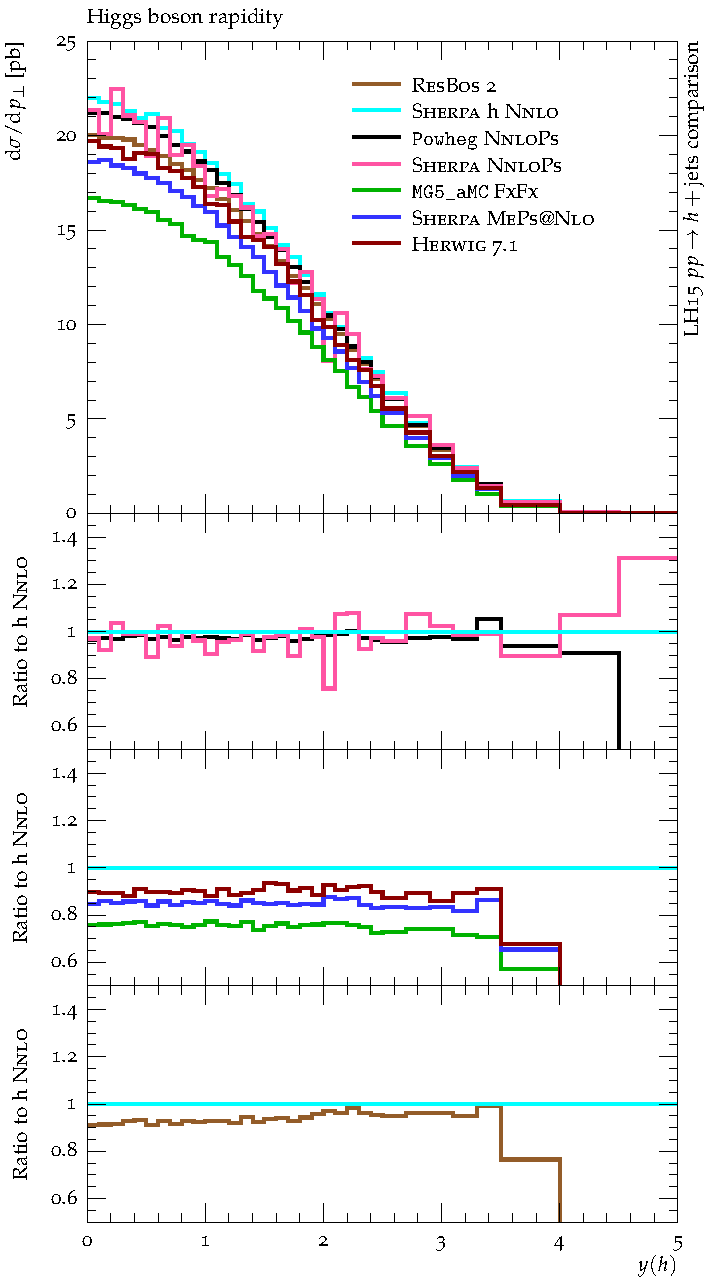
\includegraphics[width=0.47\textwidth]{figures/hjetscomp_u_H_y.pdf}
  \hfill
  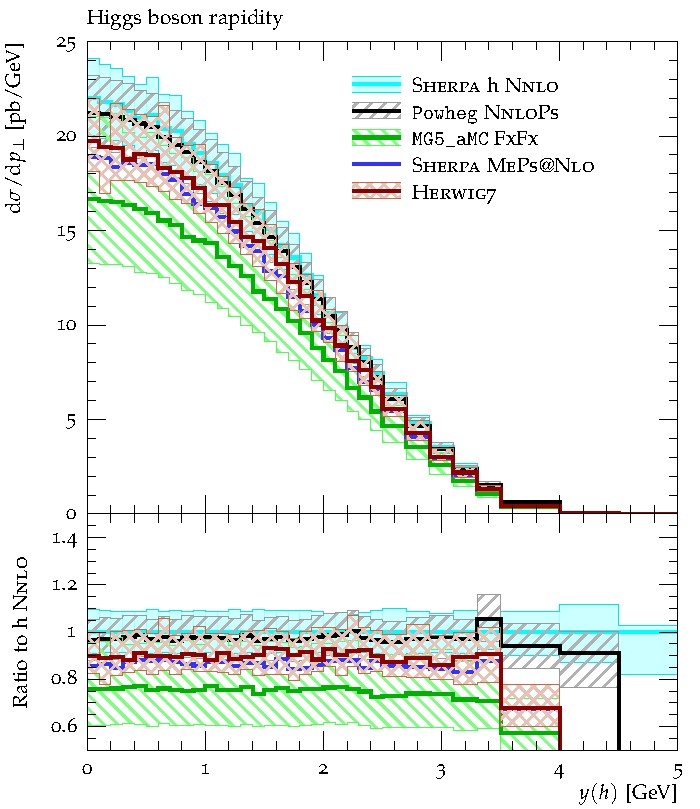
\includegraphics[width=0.47\textwidth]{figures/hjetscomp_H_y.pdf}
  \caption{\label{fig:higgscomp:results:inclobs:hy}%
    The inclusive Higgs boson rapidity without (left) and with (right)
    uncertainties. To enhance visibility, the \NNLOPS and \MEPSatNLO
    predictions are grouped together and shown with respect to the same reference
    curve in the upper and lower ratio plots, respectively. The
    reference prediction is taken from the NNLO accurate description
    of inclusive $h$ production.}
\end{figure}

We start by examining the inclusive Higgs boson rapidity distribution in
Figure~\ref{fig:higgscomp:results:inclobs:hy}. While the absolute
predictions are given in the top panel, the plots in the bottom panel
depict the respective ratios to the NNLO prediction. For better
visibility, we have divided the predictions into two groups based on
their simulation type and/or claimed accuracy. The upper ratio plot
contains the NNLO predictions while the lower one shows those obtained
from different strategies to merge matrix elements plus parton showers
at NLO. Overall, we find very good agreement in the description of the
shape of the Higgs boson rapidity distribution. The main source of deviations stems
from the different normalizations given at NNLO or NLO and the
different (core) scale choices. As expected, the \Sherpa \NNLOPS and
\Powheg \NNLOPS results agree well with the fixed order NNLO prediction. 
\Sherpa \NNLOPS' larger fluctuation wrt.\ to \Powheg \NNLOPS' stem from 
it being computed directly rather then reweighted from a NLO computation. 
Consequently, \MGaMC, \Sherpa \MEPSatNLO and \Herwig have slightly lower (NLO)
normalizations.  Here, the \MGaMC scale choice reducing to
$m_h$, rather than $\tfrac{1}{2}m_h$, is clearly noticeable. The upper edge of
the \MGaMC uncertainty band (equal to a scale that reduces to $\tfrac{1}{2}m_h$)
agrees with the central value of the other NLO ME+PS
predictions. There are no major differences in the size of the
uncertainty envelopes, although to some extent, the NNLO scale
uncertainty bands are smaller than those at NLO, as expected. Note
that the NLO-based predictions fall off more rapidly at higher $y$
than the NNLO-based predictions do. This is expected because of the
influence of additional $\ln(1-x)$ corrections present in the
determination of NNLO PDFs. Similar effects can be observed in going
from LO to NLO.

\begin{figure}[t!]
  \centering
  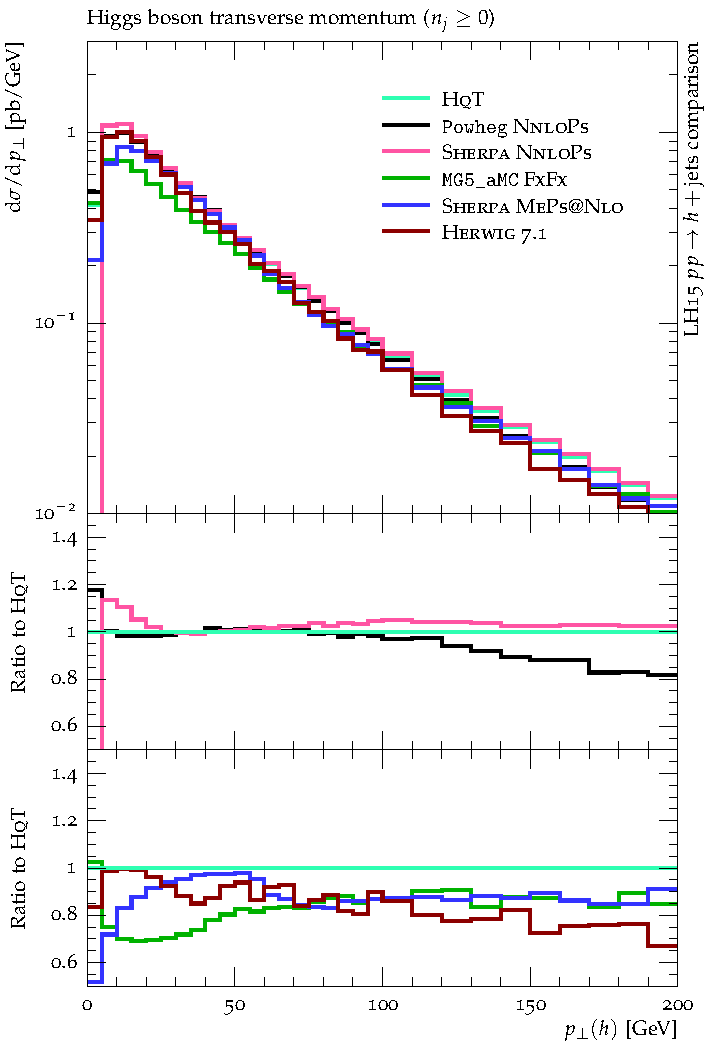
\includegraphics[width=0.47\textwidth]{figures/hjetscomp_u_H_pT_incl.pdf}
  \hfill
  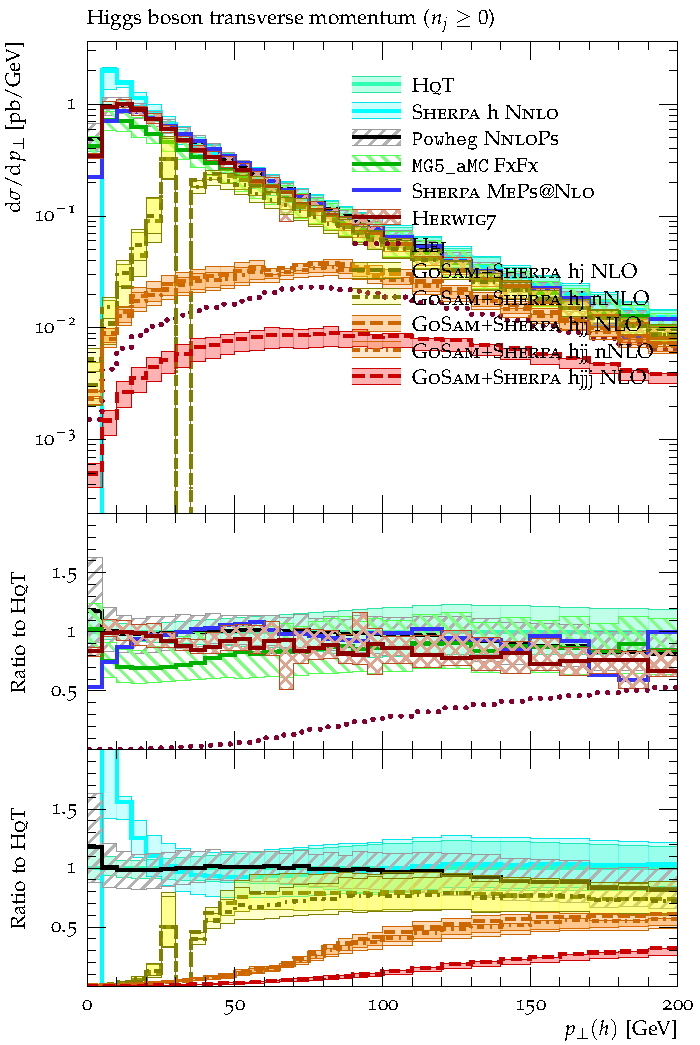
\includegraphics[width=0.47\textwidth]{figures/hjetscomp_H_pT_incl.pdf}
  \caption{\label{fig:higgscomp:results:inclobs:hpt}%
    The Higgs boson transverse momentum in the inclusive event
    selection without (left) and with (right) uncertainties. For the
    ratios in the bottom panel, the same grouping strategy has been
    used as in Figure~\ref{fig:higgscomp:results:inclobs:hy}, while
    the reference prediction has been changed from that of pure NNLO
    to the one as given by \HqT.}
\end{figure}

\begin{figure}[t!]
  \centering
  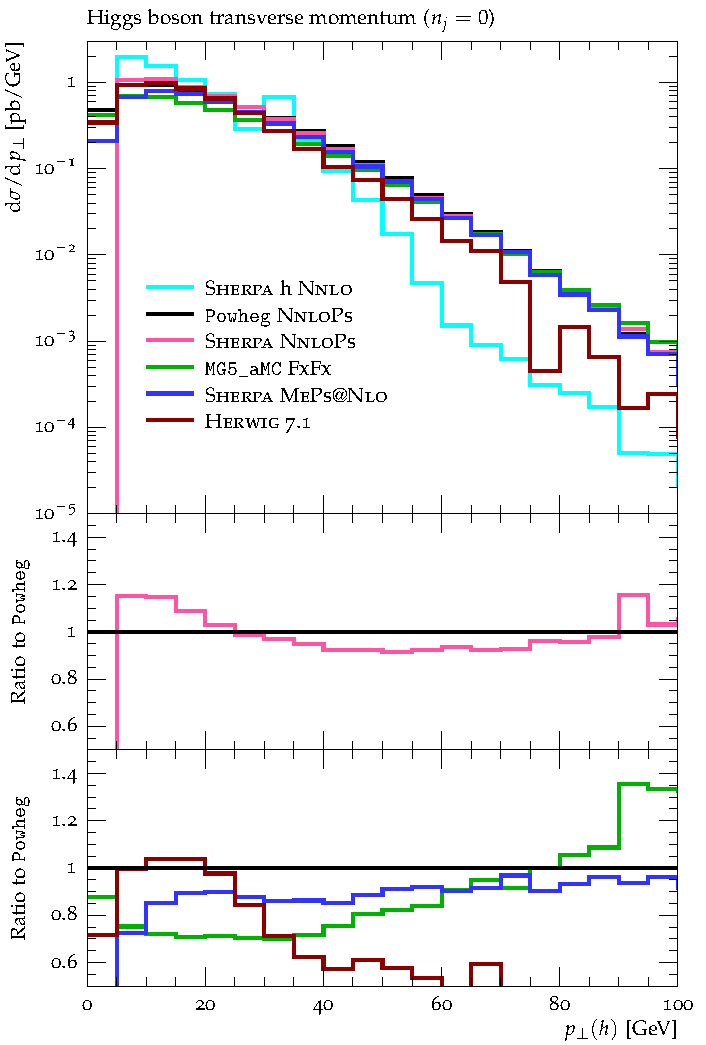
\includegraphics[width=0.47\textwidth]{figures/hjetscomp_u_H_pT_excl.pdf}
  \hfill
  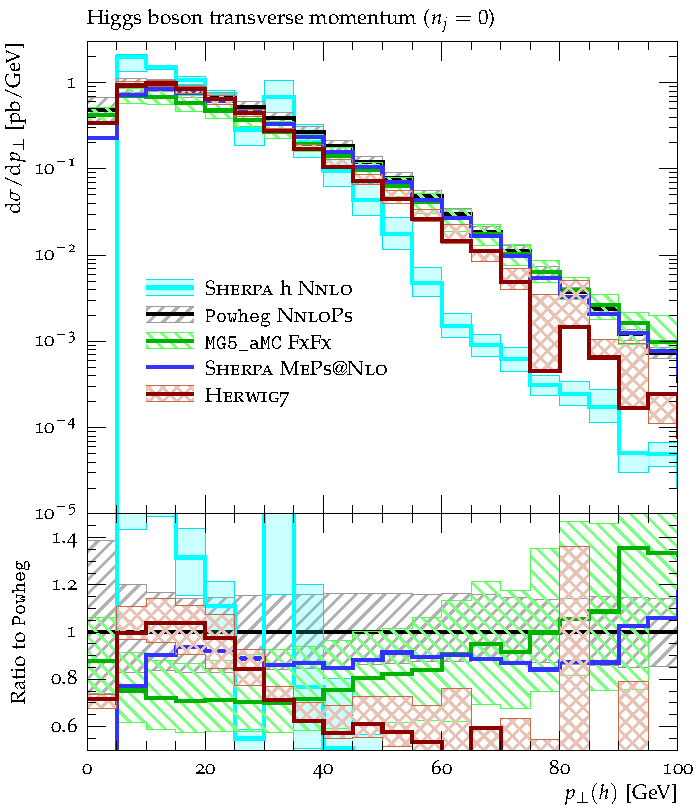
\includegraphics[width=0.47\textwidth]{figures/hjetscomp_H_pT_excl.pdf}
  \caption{\label{fig:higgscomp:results:exclobs:hpt}%
    The Higgs boson transverse momentum in the exclusive event
    selection (i.e.~in the absence of any jet) without (left) and with
    (right) uncertainties. The bottom panel has been arranged as in
    the previous figure, apart from switching to a new reference curve
    which has been obtained from \Powheg \NNLOPS.}
\end{figure}

In Figures~\ref{fig:higgscomp:results:inclobs:hpt} and
\ref{fig:higgscomp:results:exclobs:hpt}, the inclusive and exclusive
(i.e.~vetoing jets above $30$\gev) Higgs boson transverse momentum
distributions are shown, respectively.  For the former, the ratios in
the bottom panel are taken with respect to the \HqT result, while
\Powheg \NNLOPS serves as the reference for the latter case. In
general, good agreement is found, with differences being somewhat more
pronounced in the exclusive case. For the inclusive version of the
$p_\perp(h)$ observable, the good agreement is observed with \HqT,
with some larger deviations evident at very low $p_\perp$. Here the 
resummation properties of the different parton showers dominate the 
spectra of the matched and merged predictions. While the
\Sherpa \NNLOPS curve starts about 15\% higher than both \HqT and \Powheg 
\NNLOPS at low $p_\perp$ it approaches the \HqT results at high $p_\perp$ 
in the fixed-order region. At the same time, \Powheg \NNLOPS follows 
\HqT closely up to scales of $\sim m_h$. Beyond that value, the 
dynamical scale employed \Powheg \NNLOPS accounts for the ensuing 
difference. The multi-jet merged calculations, due to their similar 
scale choices, follow the pattern of the \Powheg \NNLOPS prediction.
Note that the differences in \MGaMC's central scale
choice becomes less significant as the Higgs boson transverse momentum
increases. \Herwig clearly provides the softest spectrum and \Sherpa
as well as \MGaMC predict a noticeably different shape for the Sudakov
suppression at low $p_\perp$. This is not covered by the \HqT
uncertainty envelope. We refrain from showing any fixed order
prediction here because they are neither stable nor reliable at low
$p_\perp$ in the Sudakov region where resummation effects play a 
dominant role.

As shown in Figure~\ref{fig:higgscomp:results:exclobs:hpt}, the
exclusive version of $p_\perp(h)$ exhibits deviations among the
predictions that become more sizable. The $p_\perp(h)$ distribution 
declines much faster, easily spanning three orders of magnitude 
between zero and $100$\gev. This observable is less straight forward 
than the inclusive $p_\perp$-spectrum as not only Sudakov effects 
dominate the low-$p_\perp$ region, but resummation effects are also 
entering through the veto on any jet activity. It thus necessitates 
both a proper description of small $p_\perp(h)$ region as well as 
jet production. Thus,
this is a stringent test of all predictions combining matrix elements and parton showers (ME+PS), as
the high transverse momentum of the Higgs boson is produced by a
combination of soft jets (those that are below the $30$\gev threshold)
and soft gluon radiation. Note that the comparison is now taken with respect to
\Powheg \NNLOPS. The inclusive 
NNLO calculation is shown to exemplify the failure of a fixed-order 
calculation on both accounts, and, thus, only the parton showered 
predictions are included in the study of the respective differences. 
Among them, apart from the differences already seen in the inclusive 
spectrum, both \NNLOPS calculations agree very well with one another, 
remaining within the 20\% uncertainty bands throughout the spectrum. 
While \Sherpa \MEPSatNLO remains mostly flat with respect to the \NNLOPS 
predictions, both \MGaMC and \Herwig exhibit difference in shape also 
also at larger transverse momenta. In the case
of \Herwig, they even grow larger than 40\%. 
From the resummation (i.e.~parton-shower)
point of view, all predictions are at the same level here, although
formally the \NNLOPS techniques lead to a more accurate description of
the exact zero-jet bin. The NLO merging approaches reduce to an \NLOPS
treatment in this zero-jet bin. It is however hard to infer this
formal difference from the behavior of the scale variation bands as
they are very comparable in size among all predictions. We conclude
that the deviation of the predictions probably provides us with a
better reflection of the true uncertainty.

\begin{figure}[t!]
  \centering
  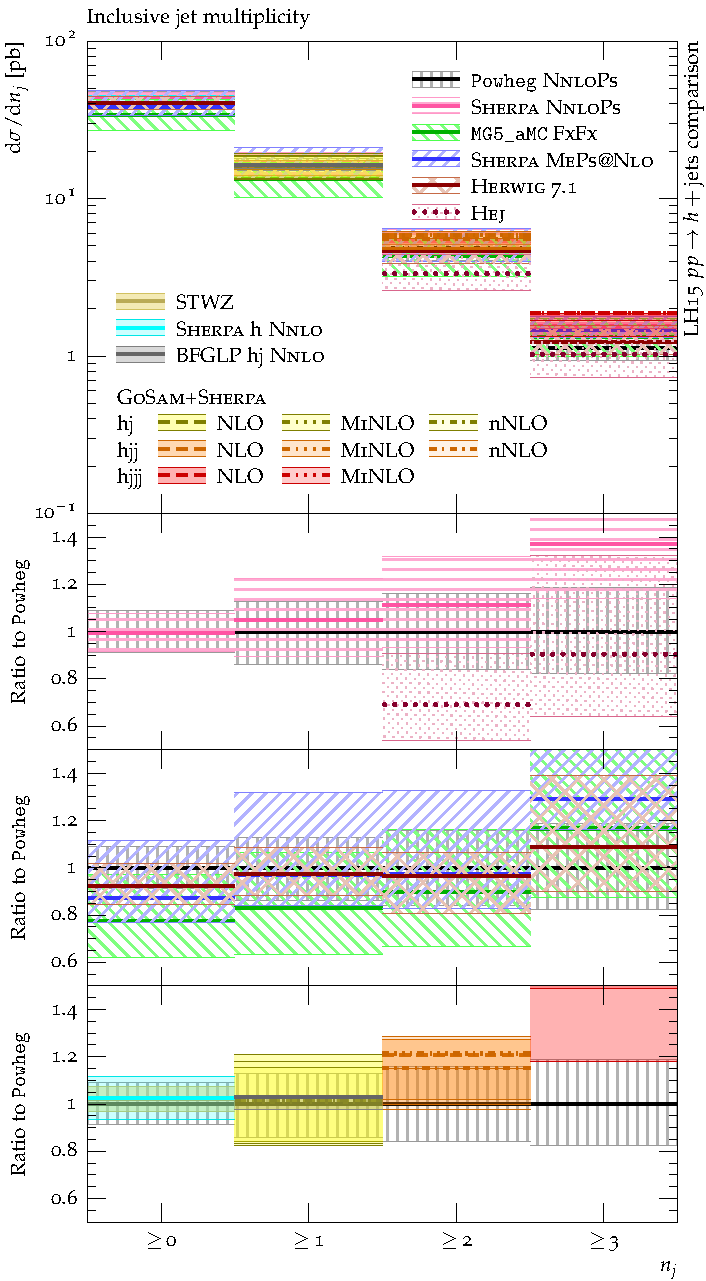
\includegraphics[width=0.47\textwidth]{figures/hjetscomp_NJet_incl_30.pdf}
  \hfill
  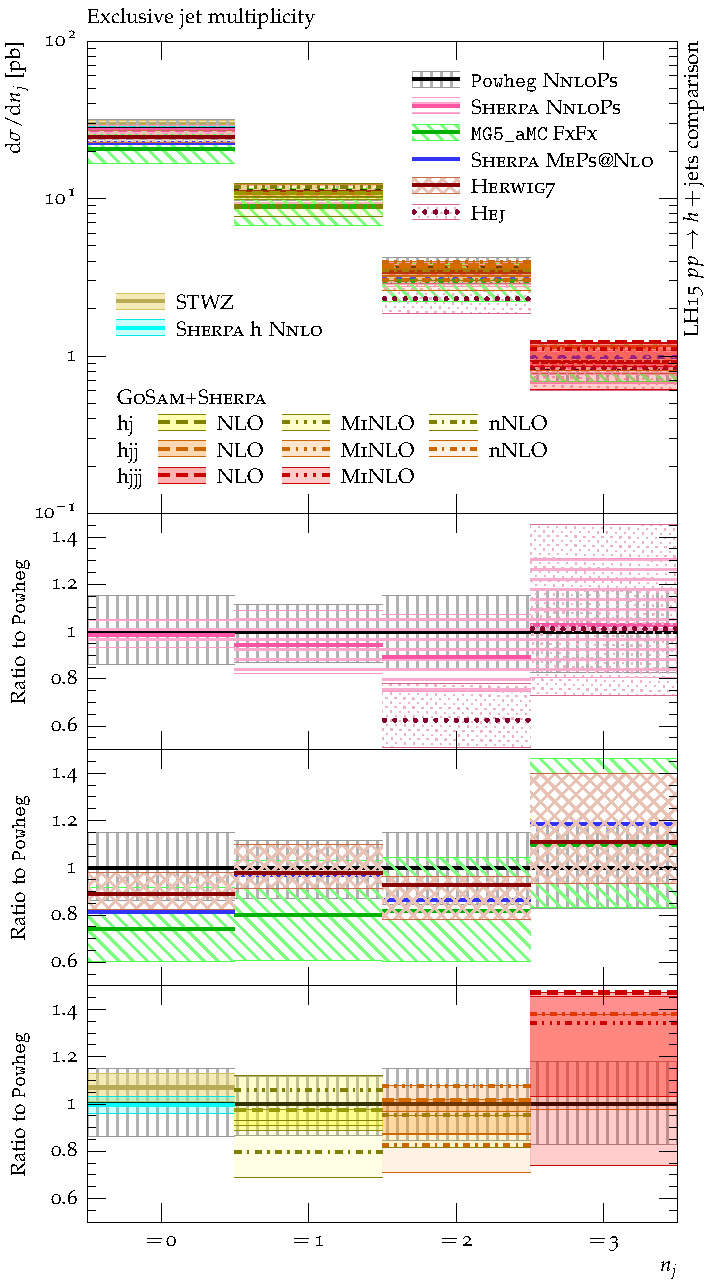
\includegraphics[width=0.47\textwidth]{figures/hjetscomp_NJet_excl_30.pdf}
  \caption{\label{fig:higgscomp:results:inclobs:njets}%
    The inclusive (left) and exclusive (right) jet multiplicities
    including theoretical uncertainties as predicted by fixed-order
    calculations, resummed calculations, NNLO and NLO Monte Carlos. The
    bottom panel is divided up into three subplots all showing the
    ratios with respect to the \Powheg \NNLOPS prediction. The upper of these plots
    contains the \Hej and \Sherpa \NNLOPS ratios, while the middle one
    includes all NLO merged predictions (\MGaMC, \Herwig and \Sherpa)
    and the lower one shows all those listed in the bottom left legend
    of the main panel.}
\end{figure}

To obtain a first impression of how the different predictions 
compare beyond the zero-jet bins ($n_j\ge0$ and $n_j=0$) we 
look at the various inclusive and exclusive $n_j$ cross sections.
Accordingly, Figure~\ref{fig:higgscomp:results:inclobs:njets} shows,
to the left, the inclusive ($n_j\ge N$) and, to the right, the
exclusive ($n_j=N$) jet multiplicity distributions up to $N=3$ 
using the previously defined \antikt jets with $p_\perp>30\gev$. Two
statements can be made before discussing the individual results in
more detail: first of all, the agreement between all results is
remarkable, and second, the details of the comparison are barely
altered when going from the inclusive description to the exclusive
description of the jet cross sections, apart from the obvious fact
that the exclusive jet bins always lie below the respective inclusive
jet bins. Although not shown here, when increasing the minimum jet-$p_\perp$ 
threshold to $50\gev$ the picture does not change significantly. 
Again, the bottom panels are split up into several ratio
plots with the common reference provided by the \Powheg \NNLOPS
results. The upper ratio plot depicts the \NNLOPS methods together
with \Hej, which only starts at $N=2$. Due to the scale choices in either 
\NNLOPS calculation they share a common inclusive cross section, with 
\Sherpa rising above \Powheg for higher jet multiplicities. Conversely,
\Hej undershoots by 30\% in the two-jet bin, where all predictions in this 
panel are LO accurate. In the three-jet bin, \Hej retains the LO accuracy 
while in both \NNLOPS calculations it is described by their respective 
parton showers only. Naturally, here the differences between the \NNLOPS 
predictions are largest. Please note, that the respective parton showering 
uncertainties are partially incorporated in the \Sherpa \NNLOPS uncertainty 
estimate while they are not assessed for \Powheg, resulting in a very flat 
uncertainty band. The central ratio plot confronts the NLO
matched and merged predictions with each other and against the common reference 
\Powheg \NNLOPS. All these predictions have claim NLO accuracy for $N=0,1,2$ 
and overlap well within uncertainties where the lower value for \MGaMC can 
again be attributed to the different scale choice. For $N=3$ only the \Sherpa 
\MEPSatNLO prediction retains its NLO accuracy while \MGaMC and \Herwig 
revert to LO, which is nicely reflected in the uncertainty estimates. 
Unsurprisingly, in the $N=3$ case, described by the reference with its 
parton shower only, all three NLO merged calculations predict larger 
cross sections.

Lastly, fixed-order predictions are shown for all jet multiplicities
at NLO (provided by \GoSam+\Sherpa) for the $1$-jet, $2$-jet and
$3$-jet bins and at approximate NNLO (labeled nNLO, provided by \Loopsim) 
for the $1$-jet and $2$-jet bins.
Complete NNLO predictions are shown for the 0-jet inclusive and
exclusive bins using \Sherpa without PS and for the 1-jet inclusive
bin using the prediction of Boughezal et al.~(BFGLP).
In addition, the zero-jet bin comparison
also contains the resummation prediction of Stewart et
al.~(STWZ) whereas the comparison for non-zero jet bins also
shows the \Minlo enhanced NLO calculations. All of the above are
grouped together in the lower ratio plot. For the zeroth bin, nice
agreement can be found between \Powheg and \Sherpa \NNLOPS as well as
the STWZ approach; the uncertainties also are of comparable
size. In the $1$-jet case, \Powheg (being NLO accurate in this bin)
resides 10\% above the pure NLO prediction, which simply is triggered
by the different scale choices. Unlike the inclusive Higgs boson
production case, the NNLO corrections for inclusive $1$-jet production
are small -- slightly negative for the central scale choice as given
in Eq.~(\ref{eq:bfglpScale}). There is a notable decrease in the scale
uncertainty with respect to the NLO band given by \GoSam+\Sherpa. The $2$-jet bin
shows the \GoSam NLO prediction just slightly above \Powheg, which
gives a LO prediction in this case. For the same reason, the \Powheg
uncertainties in the higher jet multiplicities are probably
underestimated. In the $3$-jet bin (both inclusive and exclusive), the
\GoSam+\Sherpa and \Sherpa \MEPSatNLO predictions clearly signal the absence of 
NLO corrections 
in the other predictions. The \Loopsim results for $h+j$ and
$h+jj$ are always somewhat below the respective \GoSam result
though the relatively large MC generation cut of $25$ \gev mean
the total rates predicted using \Loopsim should be interpreted with care.
Furthermore, compared to the NLO benchmark, the \Minlo approach
predicts 10-20\% larger cross sections for all non-zero jet bins.
Note that the \Minlo ratio for inclusive
$h+jjj$ turns out to be outside the plot range appearing at around
$1.65$ where the lower edge of the uncertainty band is seen kicking in
at a ratio value of $1.5$. In the cases where NNLO precision is available
the reduction in scale uncertainty is clear. For $n_j\geq1$ the variation around
$\mu_R=\sqrt{\Sigma_T}/2$ is about $5.5\%$ while for $n_j\geq0$ it is about $10\%$
around $\mu_R=m_h/2$. The latter result can be improved using the N${}^3$LO prediction
of Anastasiou et al. \cite{Anastasiou:2015ema} to only a few percent. In order to compare more
easily with results presented previously in the literature we give numerical values at NLO and NNLO
for different scale choices in Table \ref{tab:H1jXS}. As observed previously \cite{Boughezal:2015dra},
the convergence of the total cross-section is improved for scales that limit to $m_h/2$. The dynamical scale
of $\sqrt{\Sigma_T}$ defined in eq. \eqref{eq:bfglpScale} is slightly harder than the fixed scale given the
minimum jet $p_{T,j}>30$. On the other hand it is softer than $\hat{H}_T'$ defined in eq. \eqref{eq:hthatprime} which explains
the differences at NLO.

\begin{table}
  \centering
  \begin{tabular}{c||c|c|c}
    order \vphantom{$\int\limits_a^b$} & $\mu_R=\mu_F=\tfrac{1}{2}\,m_h$ & $\mu_R=\mu_F=\tfrac{1}{2}\,\hat{H}_T'$ & $\mu_R=\mu_F=\tfrac{1}{2}\,\sqrt{\vphantom{\big[}\Sigma_T}$ \\
    \hline\hline
    NLO \vphantom{$\int\limits_a^b$}  & $17.0^{+3.0}_{-2.9}$ pb & $13.5^{+2.0}_{-2.1}$ pb & $16.2^{+3.1}_{-2.8}$ pb \\\hline
    NNLO \vphantom{$\int\limits_a^b$} & -     & -     & $16.4^{+0.0}_{-0.9}$ pb \\
    \hline
  \end{tabular}
  \caption{
    The total cross-section for inclusive production of a Higgs boson and 
    one additional jet using different core scale choices.  The two 
    dynamical scales are $\hat{H}_T'=m_{T,h} + \sum_{\rm partons} p_T$ 
    (see also eq.~\eqref{eq:hthatprime}) and 
    $\Sigma_T = m_h^2 + \sum_{\rm jets} p_T^2$ 
    (see also eq.~\eqref{eq:bfglpScale}).
  }
  \label{tab:H1jXS}
\end{table}


\subsection{One-jet observables}
\label{sec:hjetscomp:results:1jobs}

\begin{figure}[t!]
  \centering
  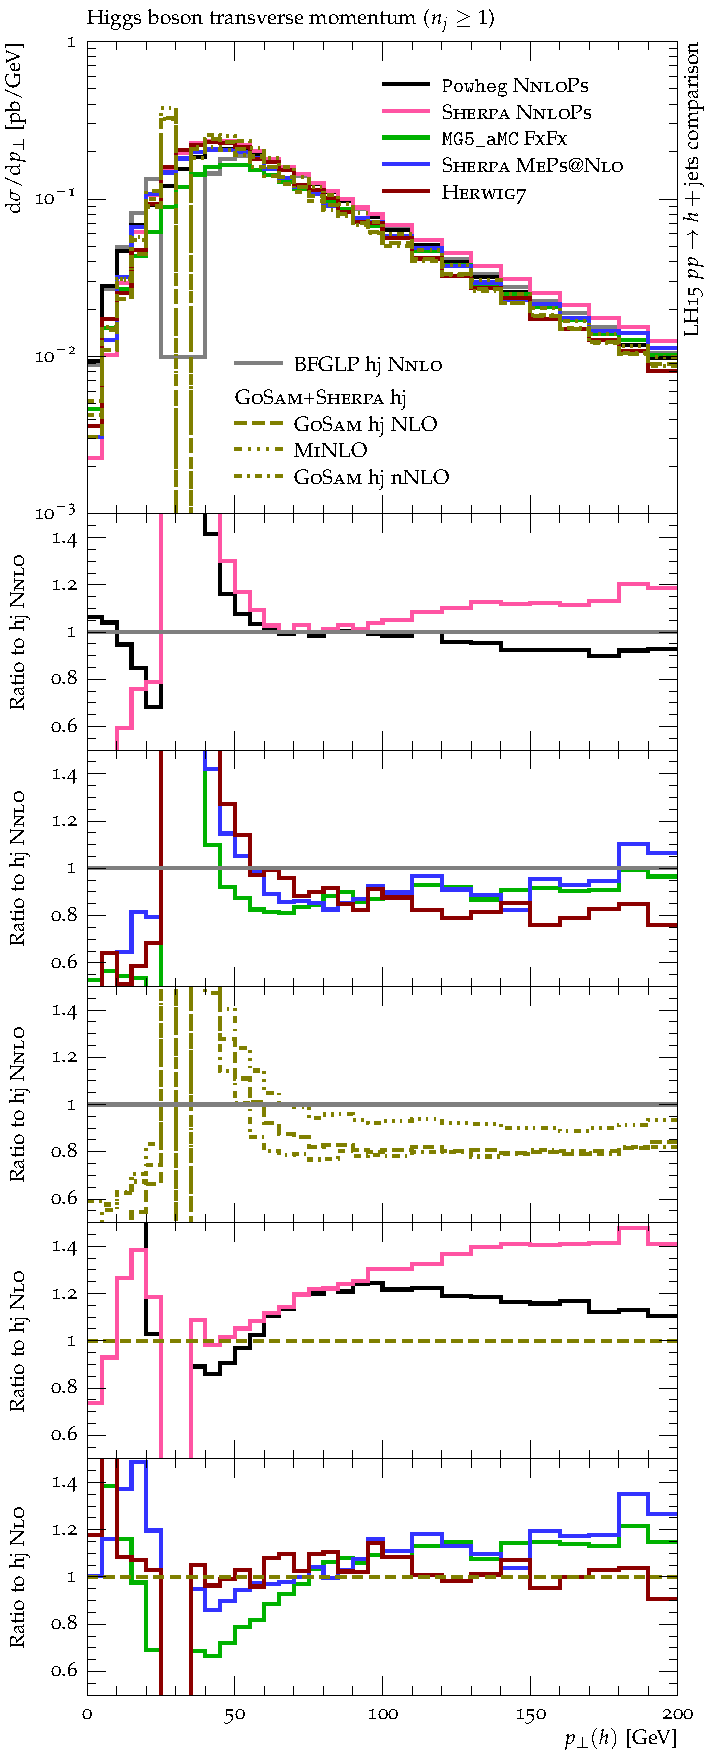
\includegraphics[width=0.47\textwidth]{figures/hjetscomp_u_H_j_pT_incl.pdf}
  \hfill
  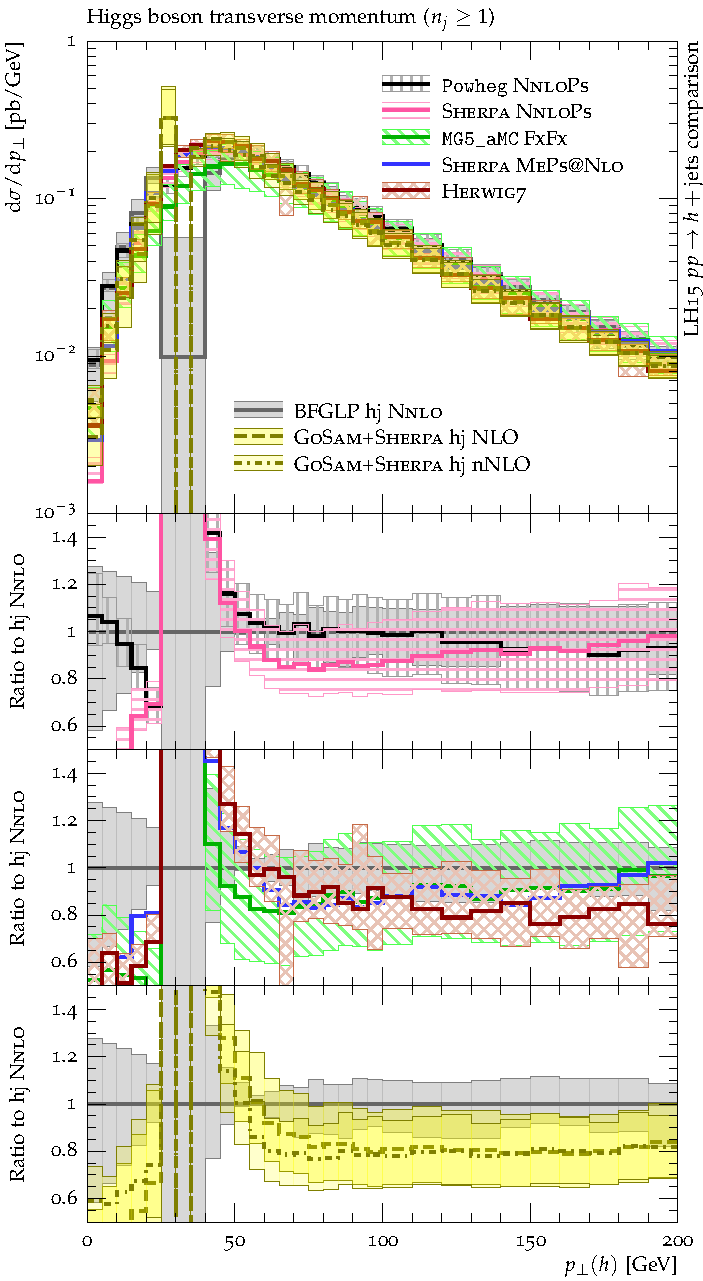
\includegraphics[width=0.47\textwidth]{figures/hjetscomp_H_j_pT_incl.pdf}
  \caption{
    The Higgs boson transverse momentum in the presence of at least
    one jet without (left) and with (right) uncertainties.
    \label{fig:higgscomp:results:1obs:hpt}
  }
\end{figure}

\begin{figure}[t!]
  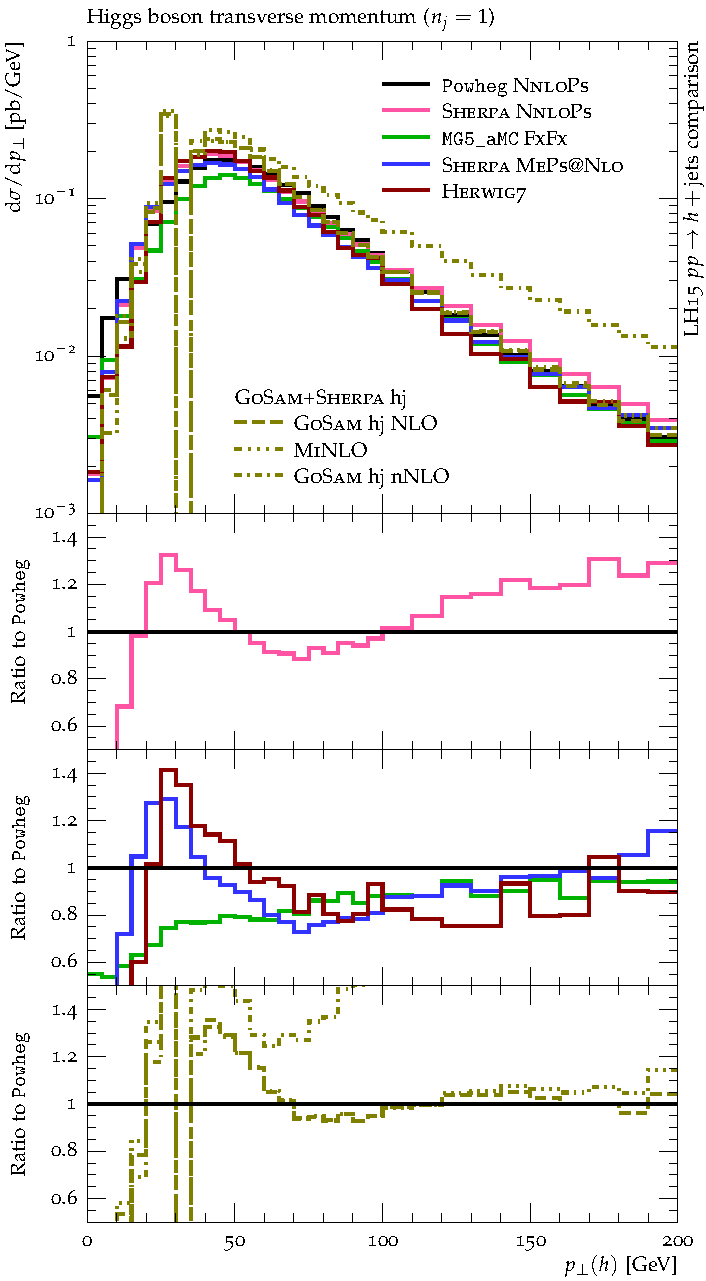
\includegraphics[width=0.47\textwidth]{figures/hjetscomp_u_H_j_pT_excl.pdf}
  \hfill
  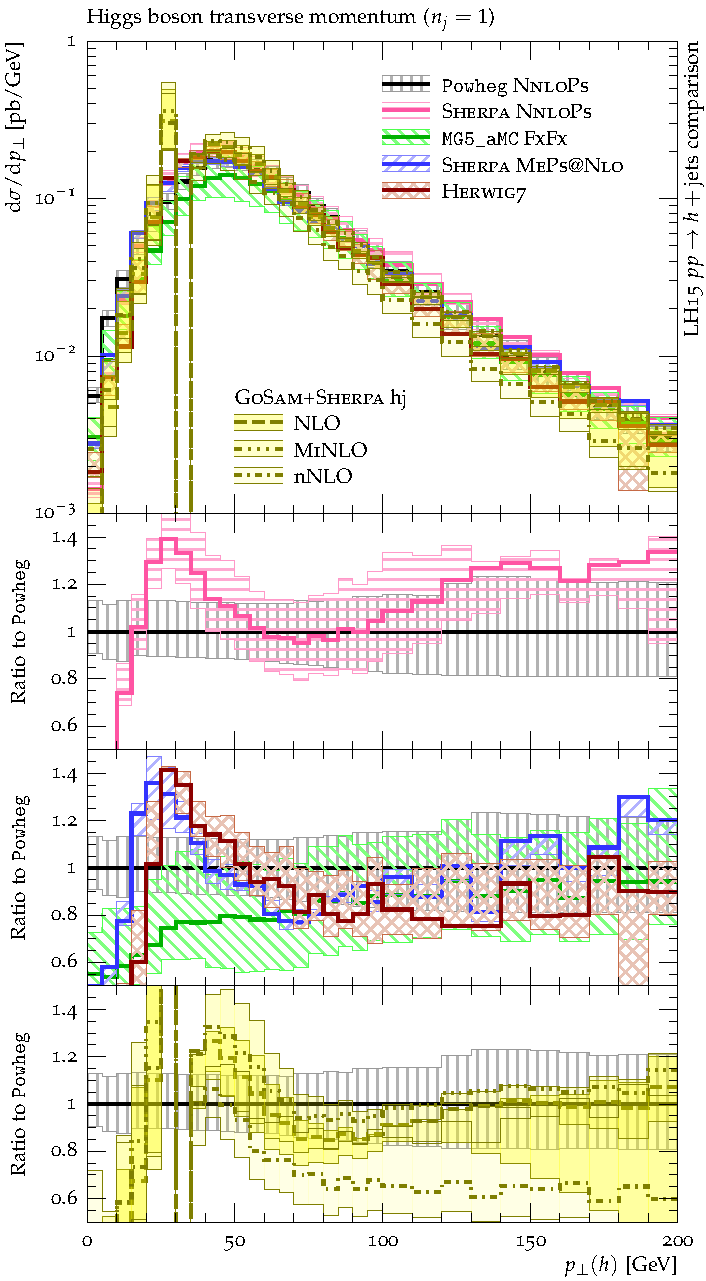
\includegraphics[width=0.47\textwidth]{figures/hjetscomp_H_j_pT_excl.pdf}
  \caption{
    The Higgs boson transverse momentum in the presence of at exactly 
    one jet without (left) and with (right) uncertainties.
    \label{fig:higgscomp:results:1obs:hpt_excl}
  }
\end{figure}

The Higgs boson transverse momentum distribution with the presence of
at least one jet is shown in
Figure~\ref{fig:higgscomp:results:1obs:hpt}. These are variables for
which large Sudakov effects are expected at low $p_T$ and indeed the
fixed order predictions are somewhat unstable for transverse momenta
less than 50 GeV/c. There are also shape differences between the ME+PS
predictions at low $p_T$. For high $p_T$, the predictions are in
better overall agreement with each other and with the NNLO
prediction. The upper edge of the MG5 error band (corresponding to the
nominal central scaler) is noticeable higher than the other
predictions.

The Higgs boson transverse momentum distribution with the presence of
exactly one jet is shown in
Figure~\ref{fig:higgscomp:results:1obs:hpt_excl}. In this case, the
differences with respect to Powheg become larger for the full
tranverse momentum range.

\Todo{concerning the two previous paragraphs $\to$ physics?}

\begin{figure}[t!]
  \centering
  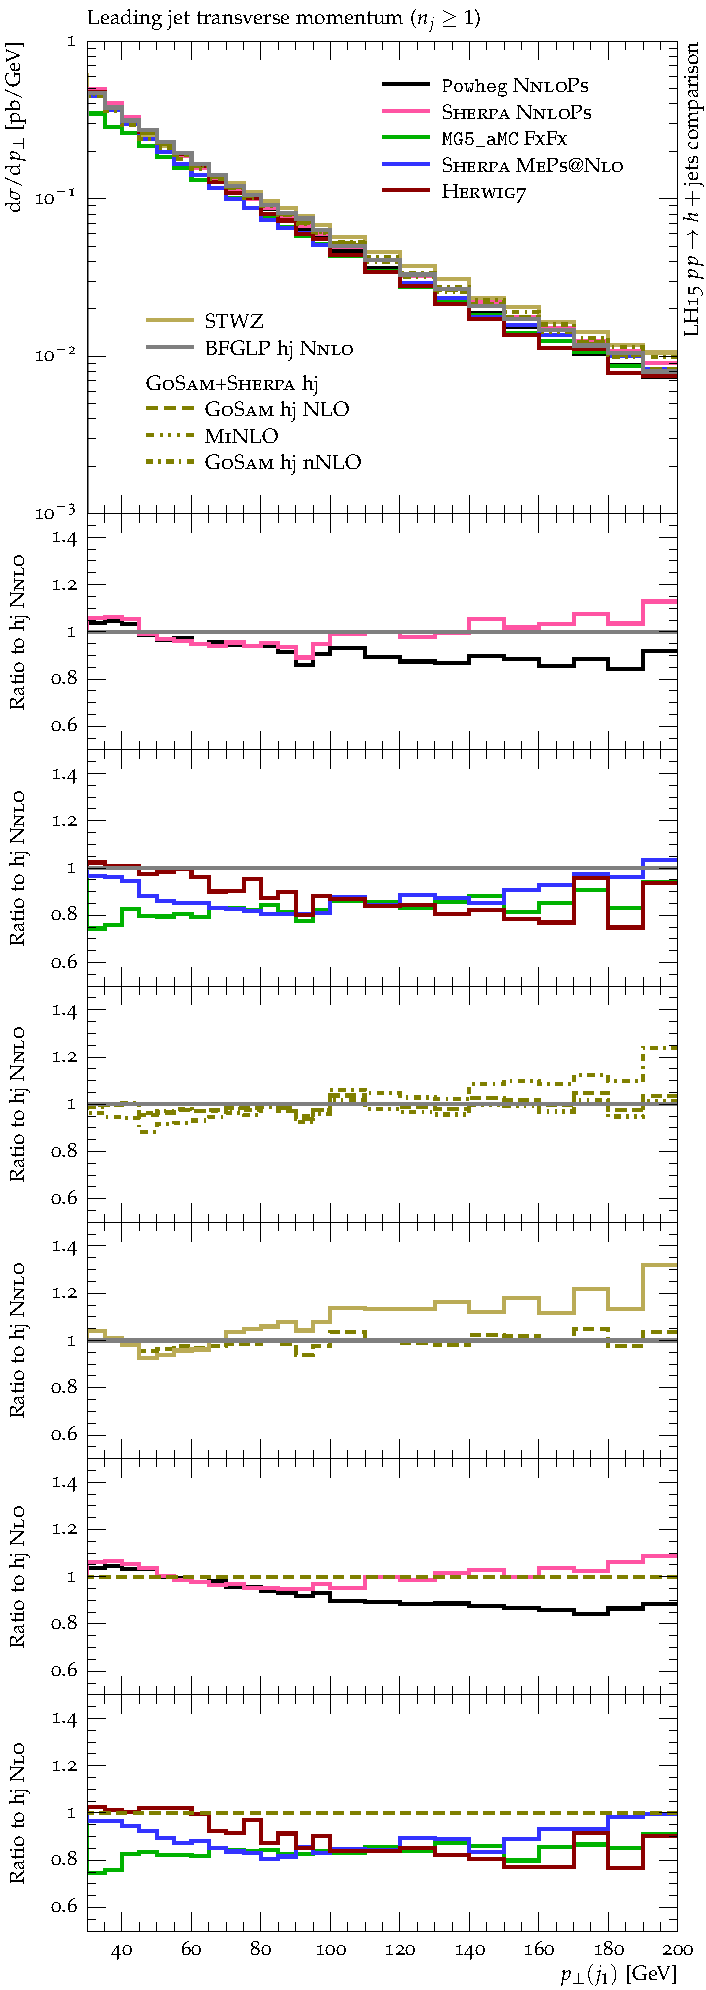
\includegraphics[width=0.47\textwidth]{figures/hjetscomp_u_jet1_pT_incl.pdf}
  \hfill
  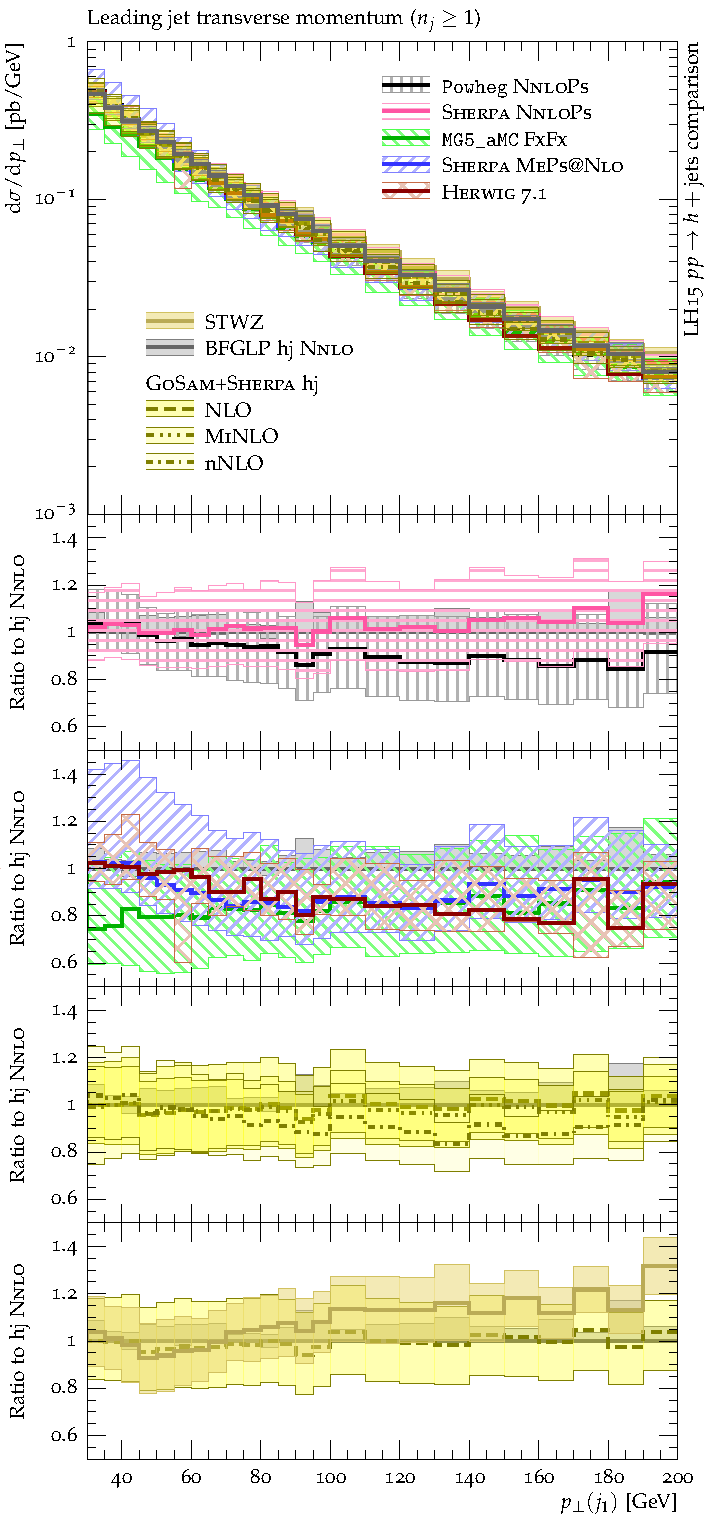
\includegraphics[width=0.47\textwidth]{figures/hjetscomp_jet1_pT_incl.pdf}
  \caption{
    The inclusive leading jet transverse momentum distribution for
    $H+\ge1$ jet production without (left) and with (right) uncertainties.
    \label{fig:higgscomp:results:1obs:j1pt}
  }
\end{figure}

The lead jet transverse momentum distribution for $H+\ge1$ jet is
shown in Figure~\ref{fig:higgscomp:results:1obs:j1pt}.

In the middle panel, the ratio of the ME+PS predictions to Powheg is
shown. Sherpa and Herwig7 have somewhat of a slope difference with
respect to Powheg in the jet transverse momentum range of 30-100
GeV/c, while MG5 (with its different central scale choice) is in
agreement with Powheg over the kinematic range shown.  In the bottom
panel, Powheg and gosam NLO and nNLO (using LoopSim) are compared (in
ratio) to the NNLO prediction for the lead jet transverse
momentum. Gosam NLO is above the NNLO prediction in the lead jet
transverse momentum range for 30-50 GeV/c, but in agreement above that
range. Powheg, with its central scale choice, is approximately 30\%
higher than the NNLO prediction for $p_T^{jet}=30$ GeV/c, and in
better agreement for $p_T^{jet}=100$ GeV/c. Thus, the central Powheg
prediction is in somewhat larger disagreement with the NNLO prediction
than with the NLO prediction in the low $p_T$ range. The nNLO
(LoopSim) prediction starts above the NNLO prediction, but then is
about 10-15\% lower for higher $p_T^{jet}$ values. The gosam MINLO
results are about 20\% higher than the nominal gosam NLO results, so
closer to Powheg at low $p_T$, but higher than Powheg at high $p_T$.

Note that for this observable, we do not expect large Sudakov effects
(i.e. shifts due to parton showering/resummation). The impact of jet
veto logarithms (due to the restriction that all jets be greater than
30 GeV/c) has been examined and found to be reasonably small at NLO
and NNLO~\cite{monni}.

\Todo{provide numbers from Monni?}
\Todo{MS: Do we have any?}

\begin{figure}[t!]
  \centering
  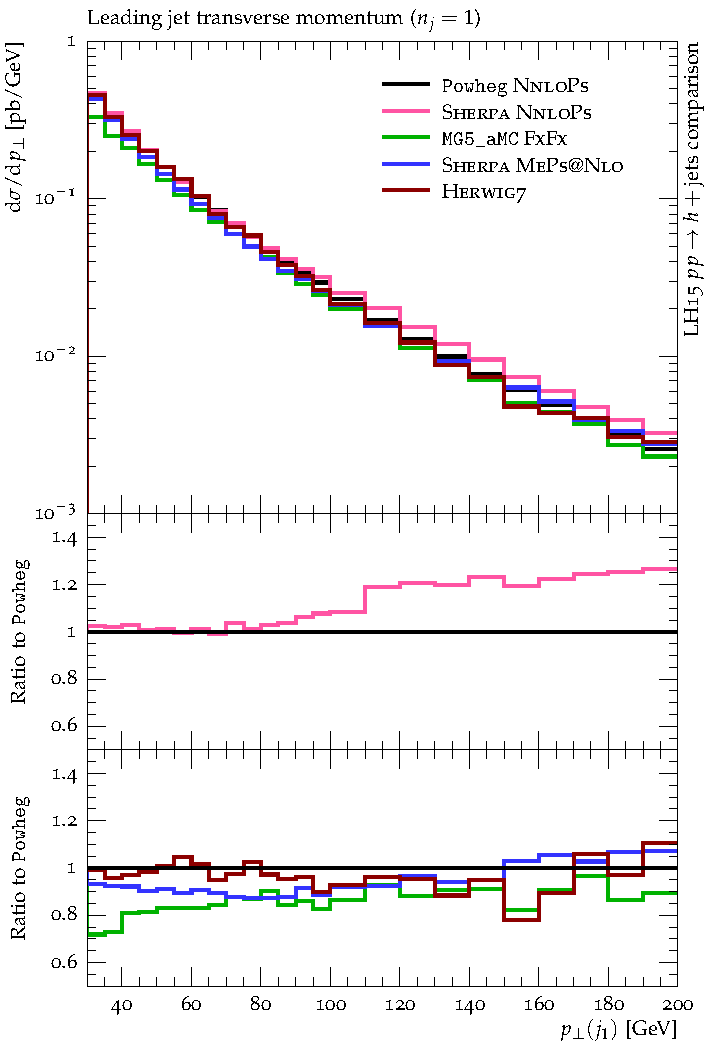
\includegraphics[width=0.47\textwidth]{figures/hjetscomp_u_jet1_pT_excl.pdf}
  \hfill
  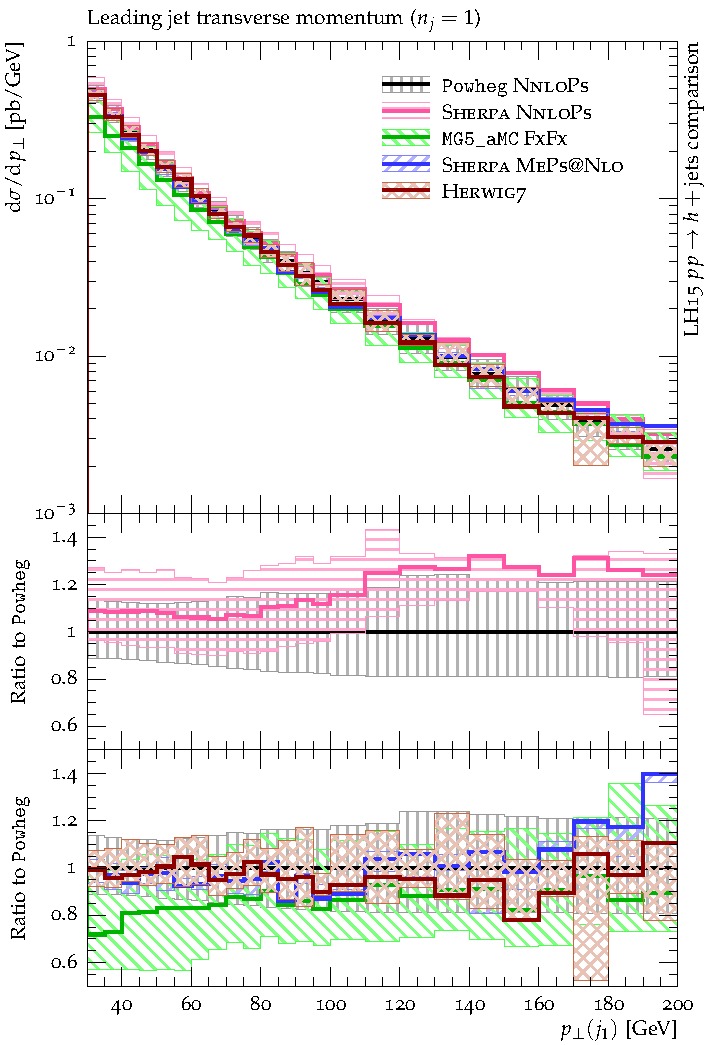
\includegraphics[width=0.47\textwidth]{figures/hjetscomp_jet1_pT_excl.pdf}
  \caption{
    The exclusive leading jet transverse momentum distribution for
    $H+\ge1$ jet production without (left) and with (right) uncertainties.
    \label{fig:higgscomp:results:1obs:j1pt_excl}
  }
\end{figure}

The exclusive lead jet transverse momentum distribution is shown in
Figure~\ref{fig:higgscomp:results:1obs:j1pt_excl}. All predictions are
in reasonably good agreement with Powheg. The MG5 prediction is lower
than Powheg for basically the entire transverse momentum range, again
because of the central scale choice. Note that this is a variable in a
strong Sudakov region, and the scale uncertainties shown do not
reflect the true uncertainty.

\begin{figure}[t!]
  \centering
  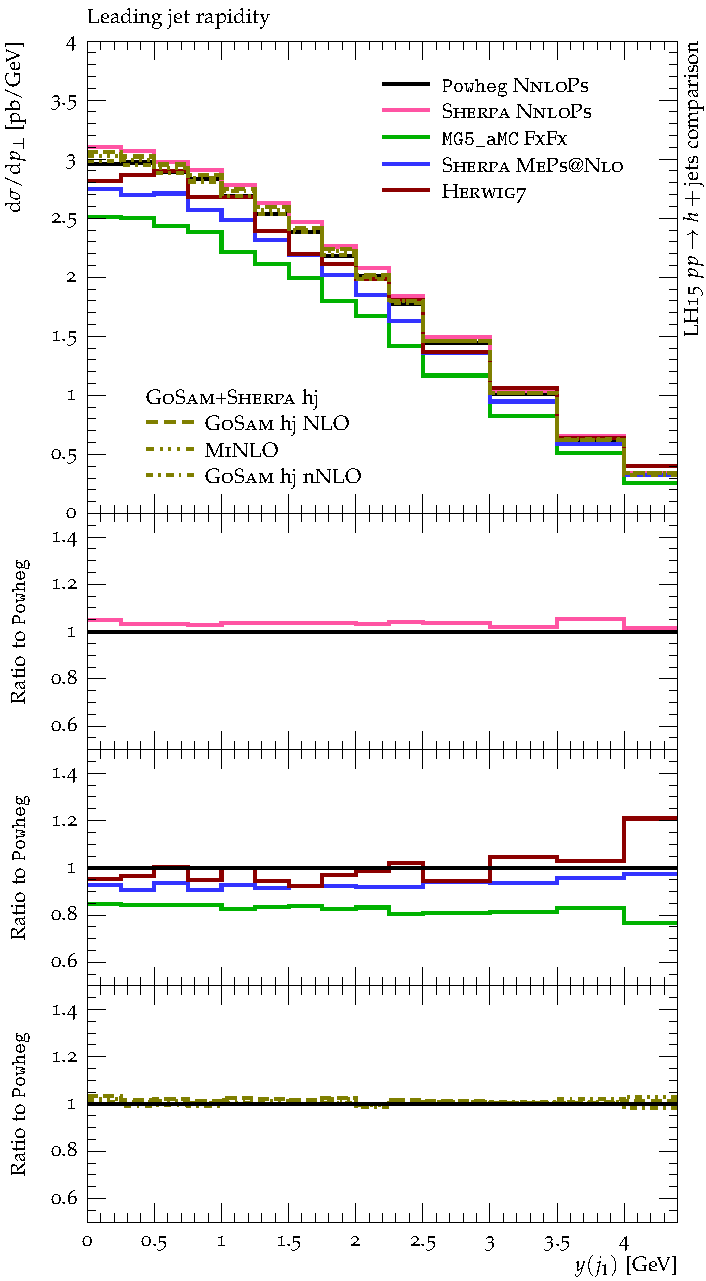
\includegraphics[width=0.47\textwidth]{figures/hjetscomp_u_jet1_y.pdf}
  \hfill
  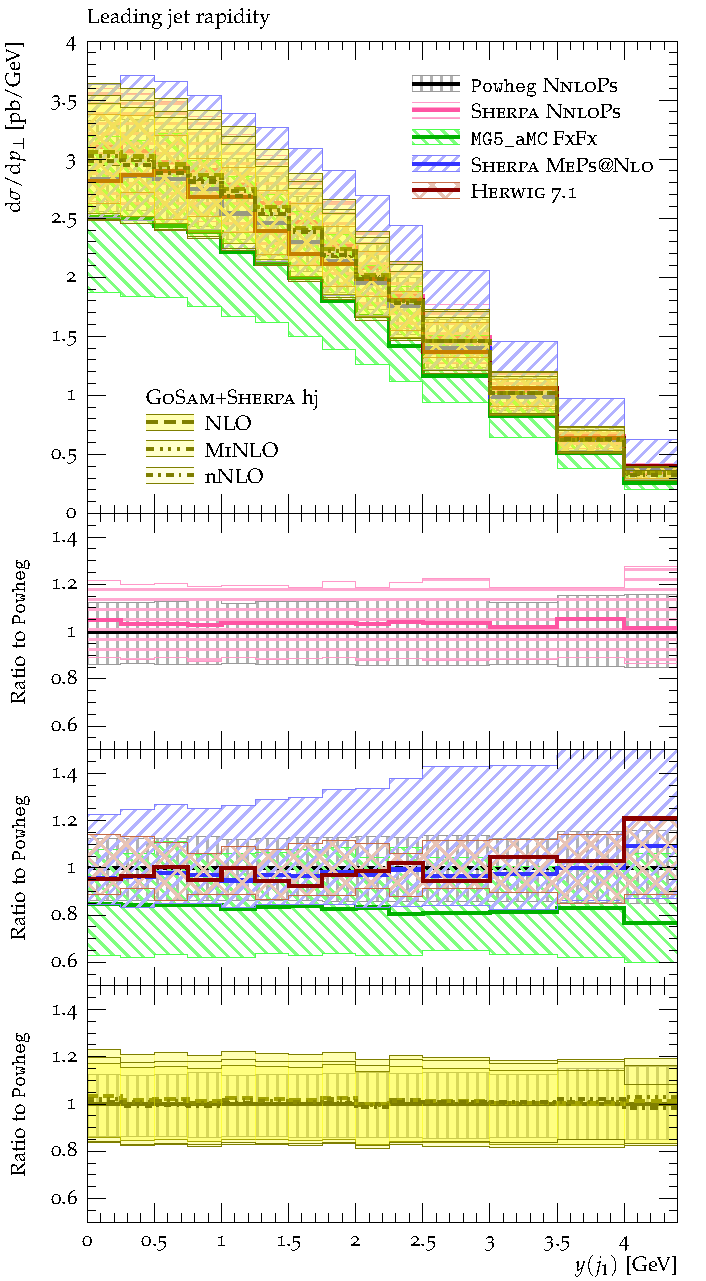
\includegraphics[width=0.47\textwidth]{figures/hjetscomp_jet1_y.pdf}
  \caption{
    The rapidity distribution for the leading jet in $H+\ge1$ jet production
    without (left) and with (right) uncertainties. 
    \label{fig:higgscomp:results:1obs:j1y}
  }
\end{figure}

The rapidity distribution for the lead jet is shown in
Figure~\ref{fig:higgscomp:results:1obs:j1y}.

\begin{figure}[t!]
  \centering
  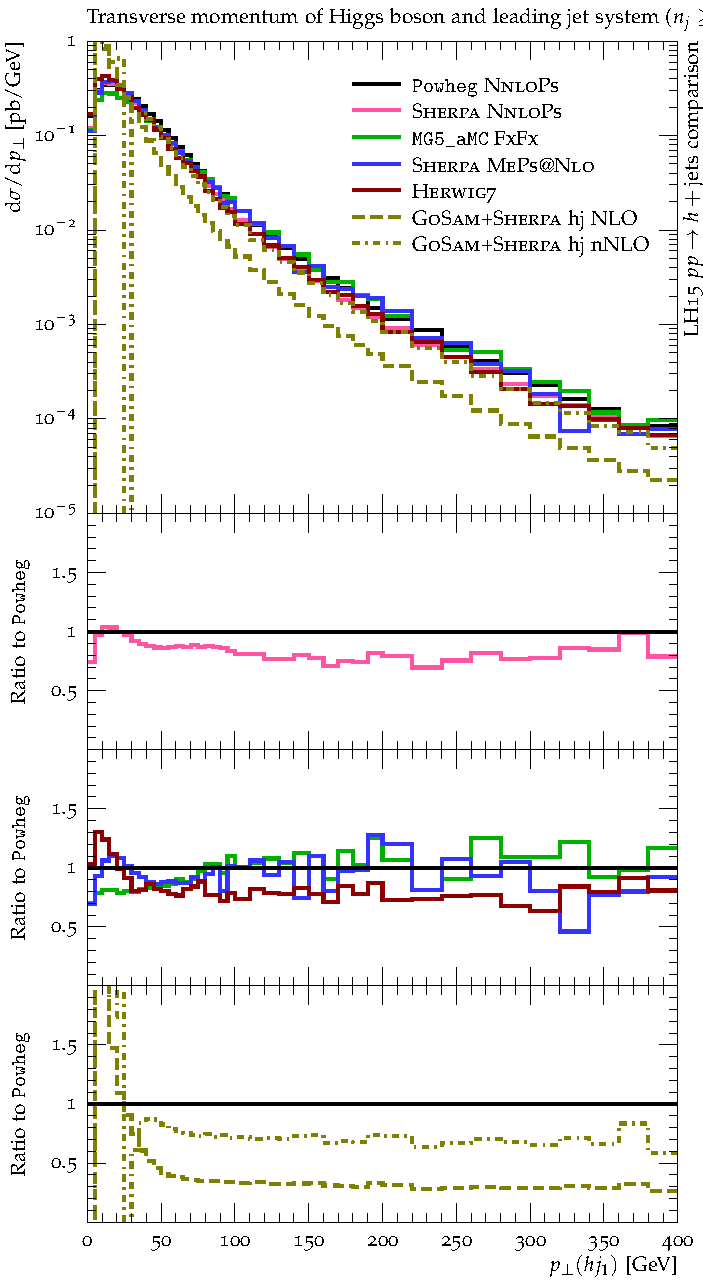
\includegraphics[width=0.47\textwidth]{figures/hjetscomp_u_Hj_pT_incl.pdf}
  \hfill
  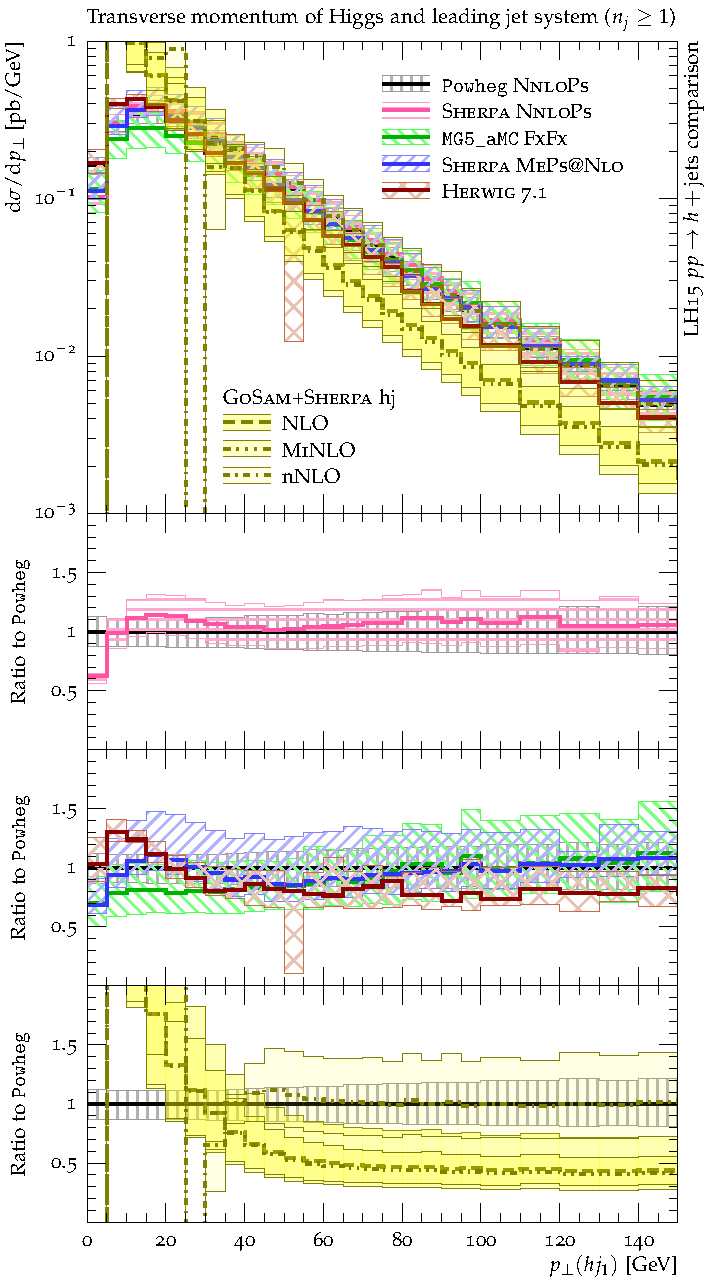
\includegraphics[width=0.47\textwidth]{figures/hjetscomp_Hj_pT_incl.pdf}
  \caption{
    The transverse momentum of the Higgs-boson-leading-jet system in the 
    presence of at least one jet without (left) and with (right) uncertainties.
    \label{fig:higgscomp:results:1obs:hj_pt}
  }
\end{figure}

\begin{figure}[t!]
  \centering
  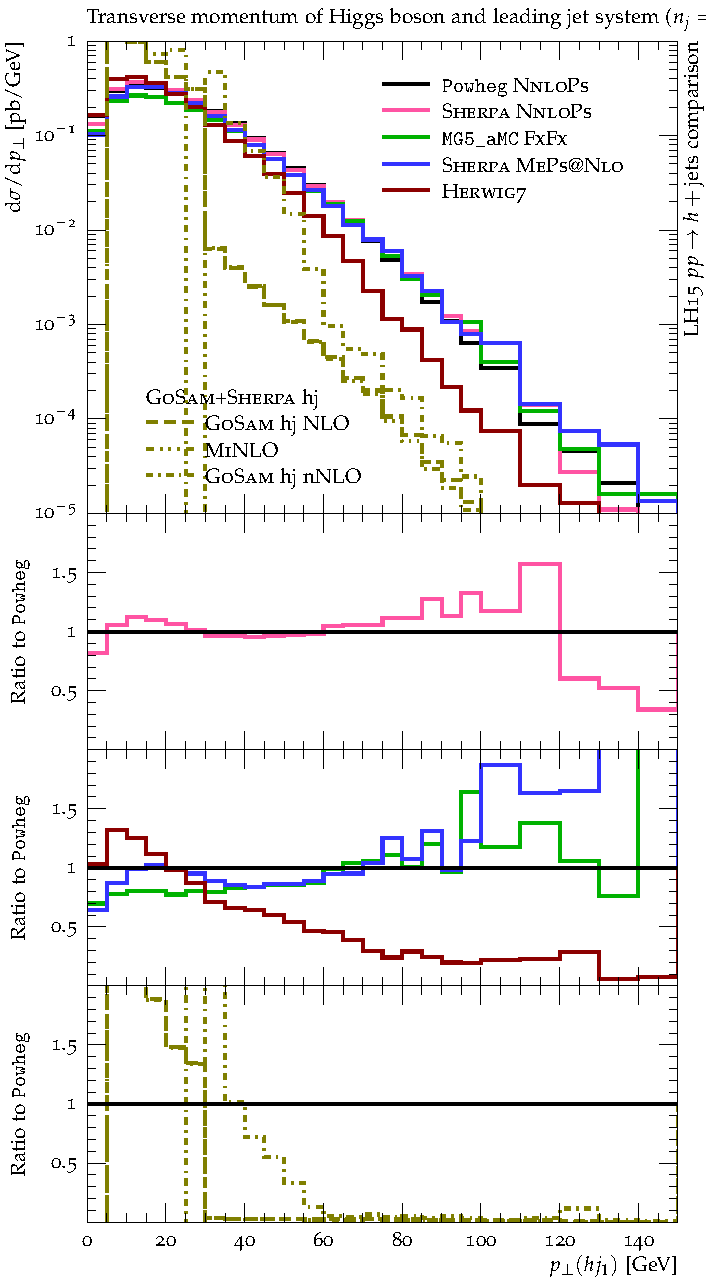
\includegraphics[width=0.47\textwidth]{figures/hjetscomp_u_Hj_pT_excl.pdf}
  \hfill
  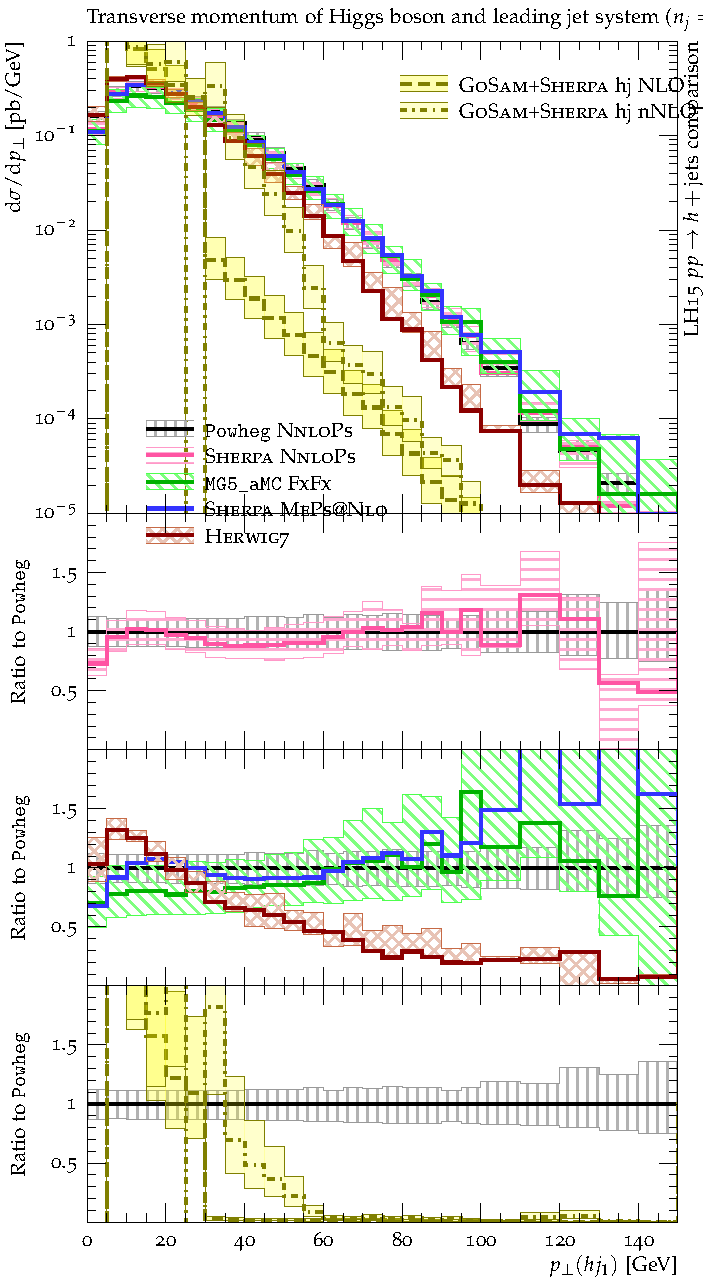
\includegraphics[width=0.47\textwidth]{figures/hjetscomp_Hj_pT_excl.pdf}
  \caption{
    The transverse momentum of the Higgs-boson-leading-jet system in the 
    presence of exactly one jet without (left) and with (right) uncertainties.
    \label{fig:higgscomp:results:1obs:hj_pt_excl}
  }
\end{figure}

Next we examine the transverse momentum of the Higgs boson + leading
jet system. The inclusive case ($\ge 1$ jet) is shown in the upper
part of Figure~\ref{fig:higgscomp:results:1obs:hj_pt}.  Again,
differences can be observed for the $\ge 1$ jet ME+PS predictions at
low $p_T$, while there is better agreement at higher $p_T$.

\Todo{but what is happening with MG5 at high pT}

The exclusive case (exactly jet) is shown in the lower part of
Figure~\ref{fig:higgscomp:results:1obs:hj_pt}.  There is a much
greater divergence of the predictions for exactly one jet, especially
at high $p_T$.  A highly exclusive distribution such as this serves as
a stress test for ME+PS prediction, similar to the case for the Higgs
$p_T$ distribution with no jets and it is no surprise that different
approaches can lead to different answers.



\clearpage
\subsection{Dijet observables}
\label{sec:hjetscomp:results:2jobs}

\begin{figure}[t!]
  \centering
  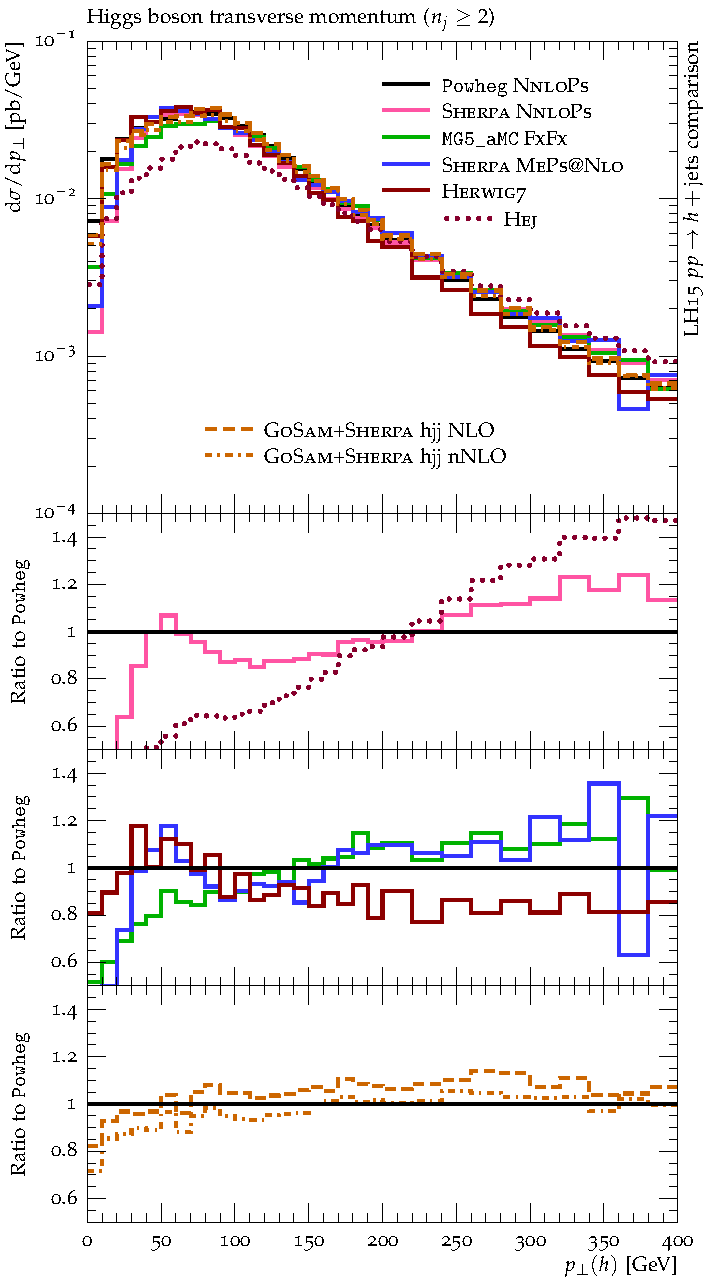
\includegraphics[width=0.47\textwidth]{figures/hjetscomp_u_H_jj_pT_incl.pdf}
  \hfill
  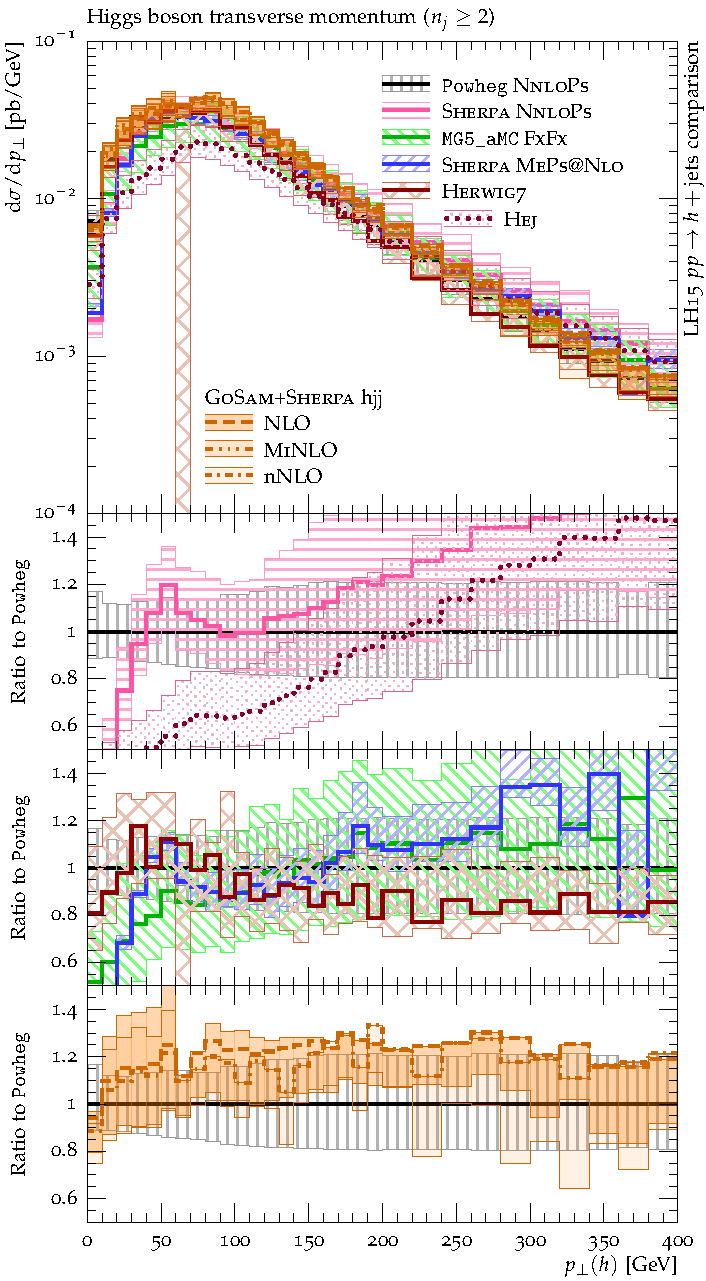
\includegraphics[width=0.47\textwidth]{figures/hjetscomp_H_jj_pT_incl.pdf}
  \caption{
    The transverse momentum of the Higgs boson in the presence
    of at least two jets without (left) and with (right) uncertainties.
    \label{fig:higgscomp:results:2obs:hpt_j2pt}
  }
\end{figure}

The Higgs boson $p_T$, in the presence of at least two jets, is shown
in Figure~\ref{fig:higgscomp:results:2obs:hpt_j2pt}. Here, varying
behavior is observed, with MG5 and Sherpa being substantially lower
than Powheg at low $p_T$ and somewhat higher at high $p_T$, while
Herwig7 is somewhat lower than Powheg at high $p_T$. The gosam
$H+\ge2$ jet prediction is lower than Powheg at low $p_T$ (as expected
for a Sudakov region),and roughly 10\% higher at high $p_T$ (closer to
the MG5/Sherpa predictions).

\begin{figure}[t!]
  \centering
  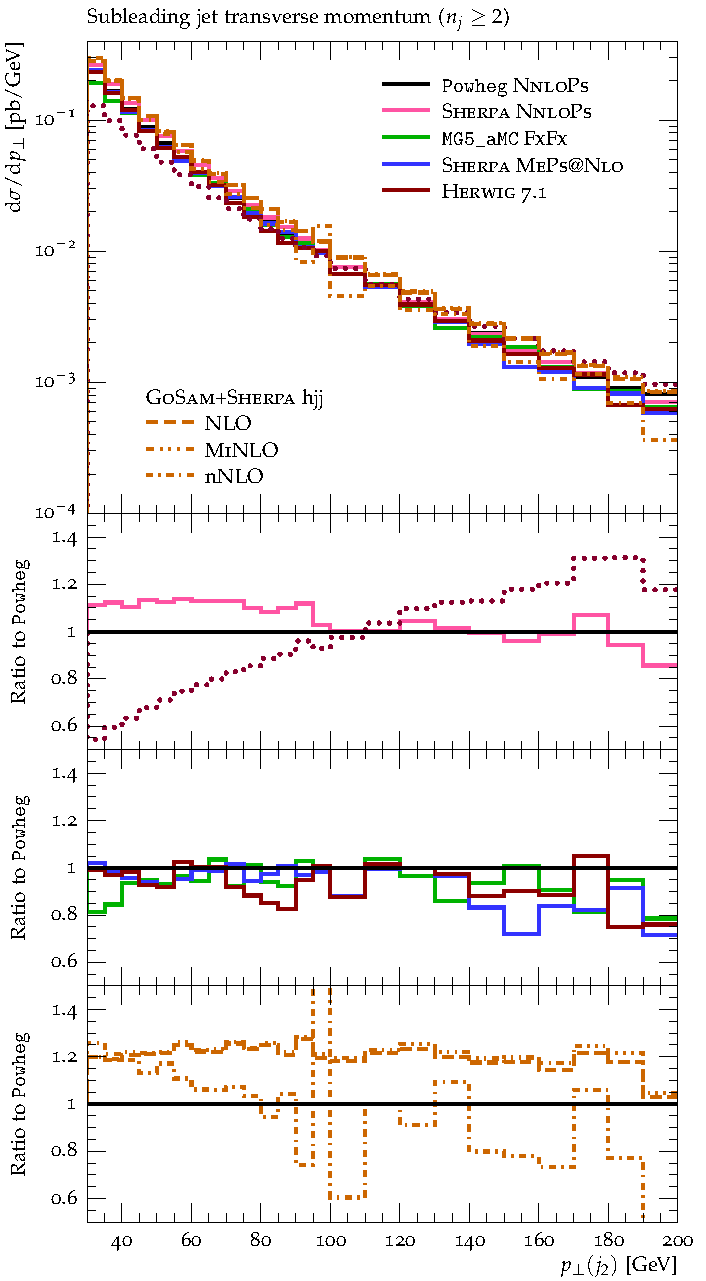
\includegraphics[width=0.47\textwidth]{figures/hjetscomp_u_jet2_pT_incl.pdf}
  \hfill
  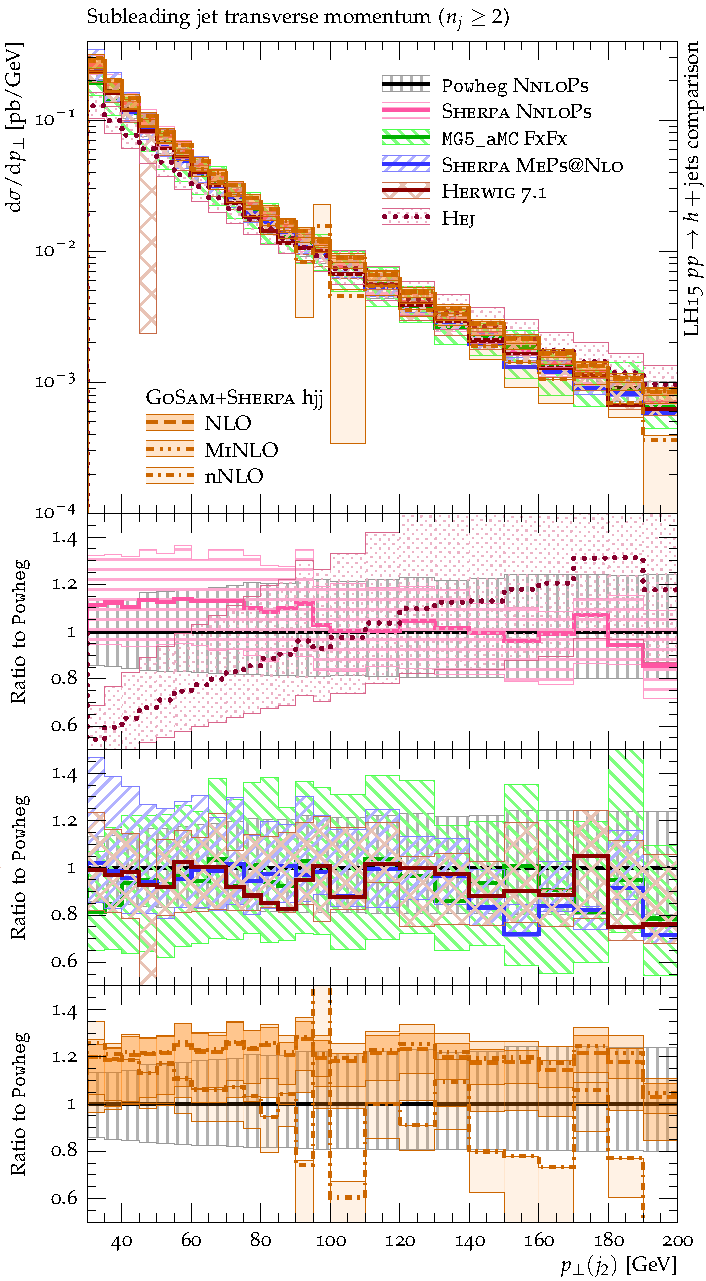
\includegraphics[width=0.47\textwidth]{figures/hjetscomp_jet2_pT_incl.pdf}
  \caption{
    The sub-leading jet $p_T$ for $H+\ge2$ jets production without
    (left) and with (right) uncertainties.
    \label{fig:higgscomp:results:2obs:jet2_pt}
  }
\end{figure}

\begin{figure}[t!]
  \centering
  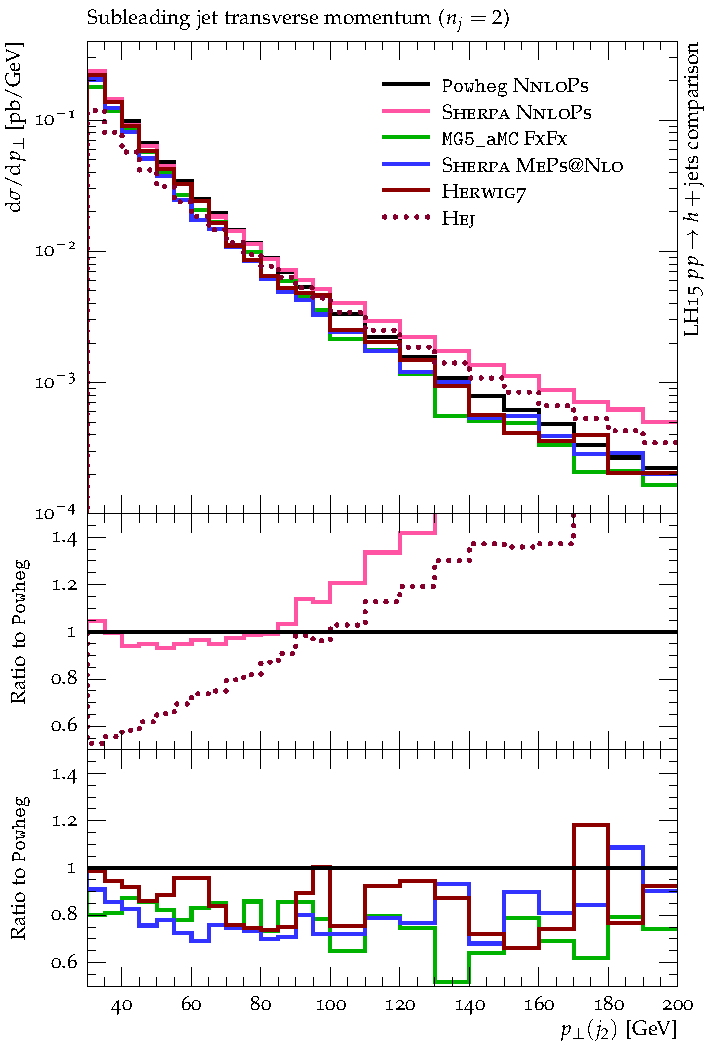
\includegraphics[width=0.47\textwidth]{figures/hjetscomp_u_jet2_pT_excl.pdf}
  \hfill
  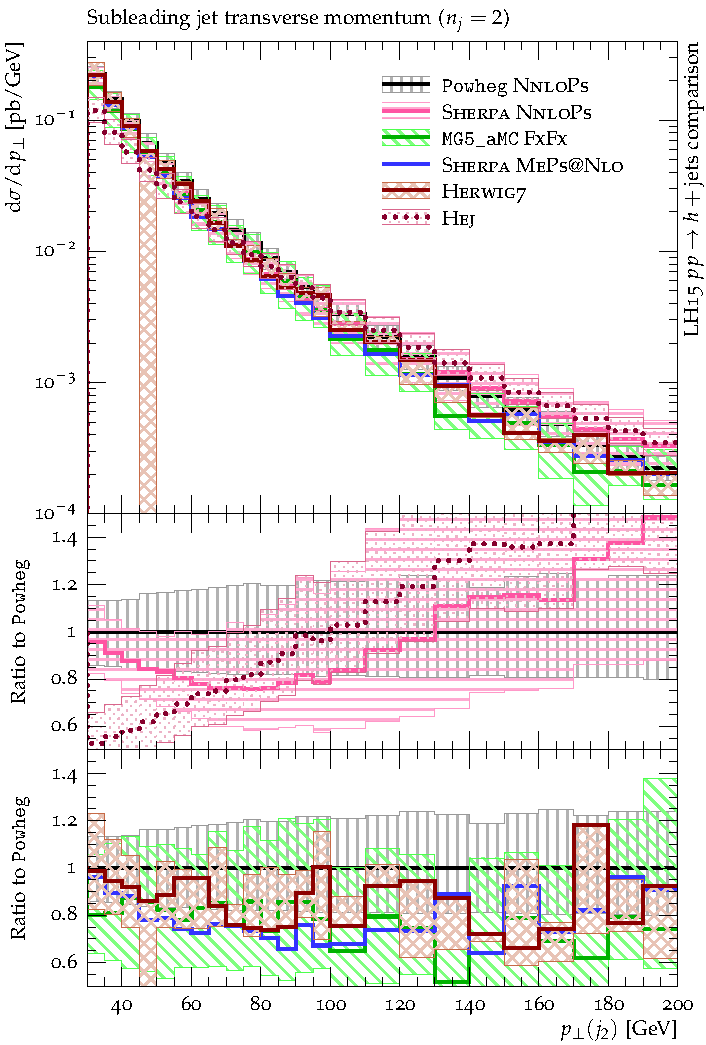
\includegraphics[width=0.47\textwidth]{figures/hjetscomp_jet2_pT_excl.pdf}
  \caption{
    The sub-leading jet $p_T$ for $H$ + exactly 2 jets production without
    (left) and with (right) uncertainties.
    \label{fig:higgscomp:results:2obs:jet2_pt}
  }
\end{figure}

The sub-leading jet $p_T$ for $H+\ge2$ jets is shown in the upper row
of Figure~\ref{fig:higgscomp:results:2obs:jet2_pt}.  The agreement
among the ME+PS predictions and between the ME+PS and fixed order
predictions of gosam is better than in the case of the leading
jets. With two or more jets in the final state, meaningful predictions
to HEJ can be made for the first time.

The sub-leading jet $p_T$ for $H$ + exactly 2 jets is shown in the
lower panel of Figure~\ref{fig:higgscomp:results:2obs:jet2_pt}.
Here, MG5, Sherpa and Herwig7 lie in reasonable agreement with each
other, but systematically lower than Powheg.

\Todo{physics?}

\begin{figure}[t!]
  \centering
  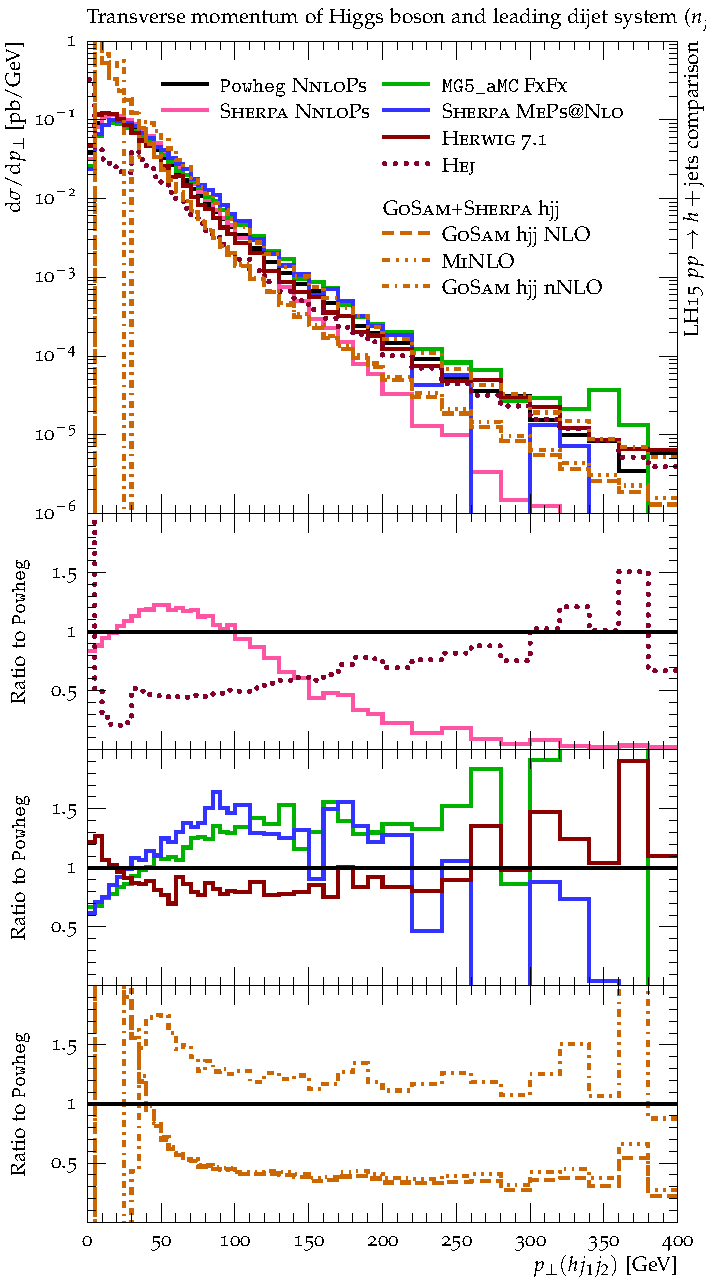
\includegraphics[width=0.47\textwidth]{figures/hjetscomp_u_Hjj_pT_incl.pdf}
  \hfill
  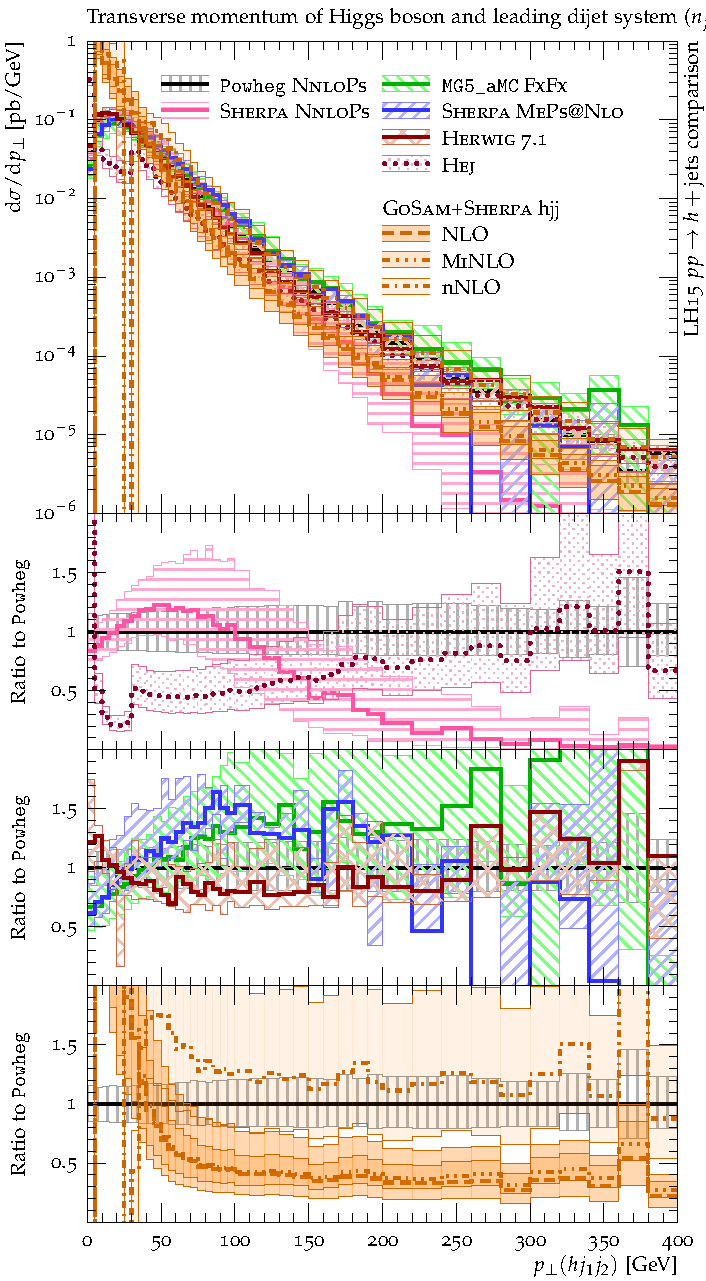
\includegraphics[width=0.47\textwidth]{figures/hjetscomp_Hjj_pT_incl.pdf}
  \caption{
    The transverse momentum of the Higgs boson plus two leading jet
    system without (left) and with (right) uncertainties.
    \label{fig:higgscomp:results:2obs:hjj_pt}
  }
\end{figure}

The transverse momentum of the Higgs boson plus two leading jet system
is shown in Figure~\ref{fig:higgscomp:results:2obs:hjj_pt}. Varying
behavior is also observed here, with MG5 and Sherpa being having a
slope with respect to Powheg at low $p_T$ and being somewhat higher at
high $p_T$, while Herwig7 is again somewhat lower than Powheg at high
$p_T$. The gosam $H+\ge2$ jet prediction is much higher than Powheg at
low $p_T$, and significantly lower at high $p_T$.

\Todo{physics!; why does gosam have the behavior it does?}

\begin{figure}[t!]
  \centering
  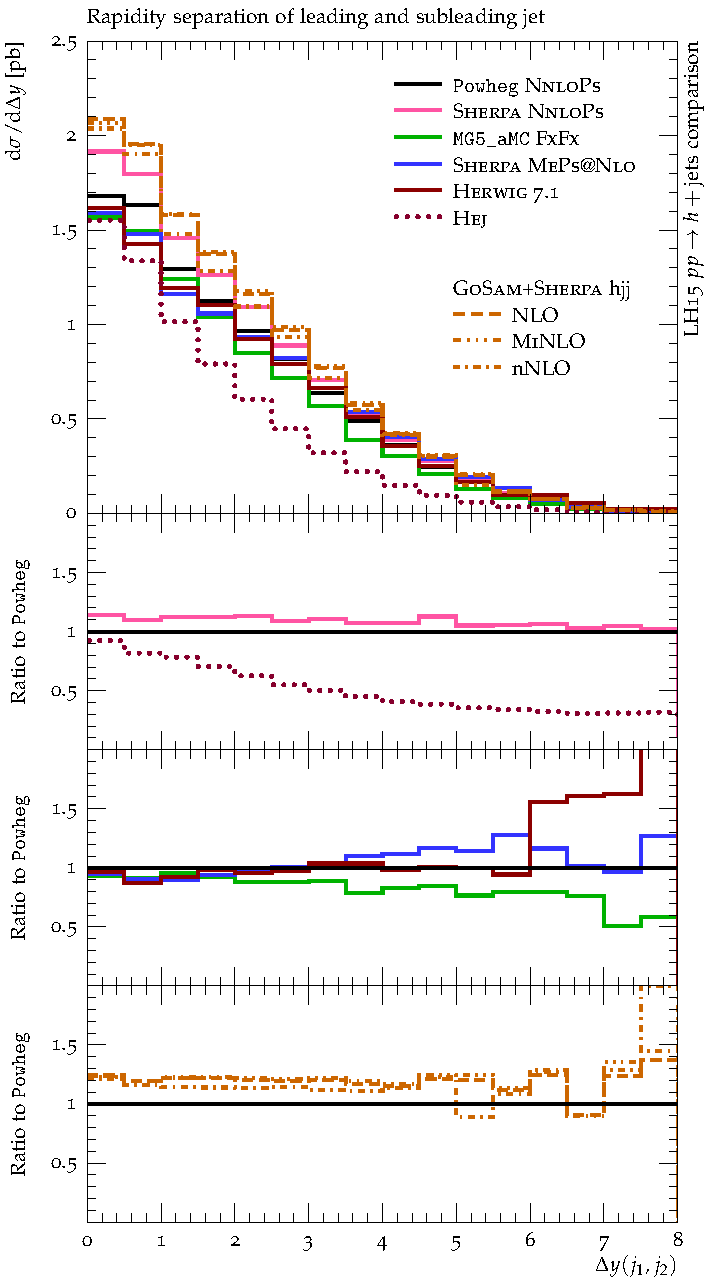
\includegraphics[width=0.47\textwidth]{figures/hjetscomp_u_deltay_jj.pdf}
  \hfill
  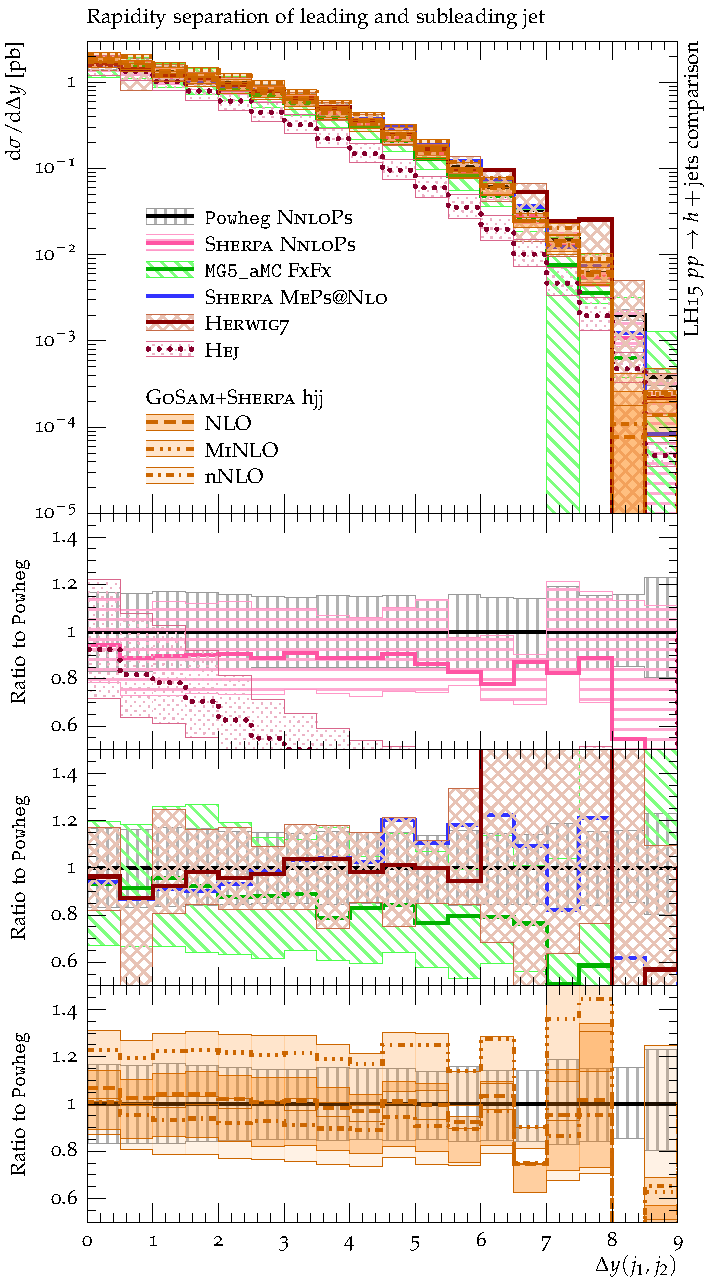
\includegraphics[width=0.47\textwidth]{figures/hjetscomp_deltay_jj.pdf}
  \caption{
    The rapidity separation between the leading and sub-leading jets
    for $H+\ge2$ jets, without (left) and with (right) uncertainties.
    \label{fig:higgscomp:results:2obs:dyjj}
  }
\end{figure}

\begin{figure}[t!]
  \centering
  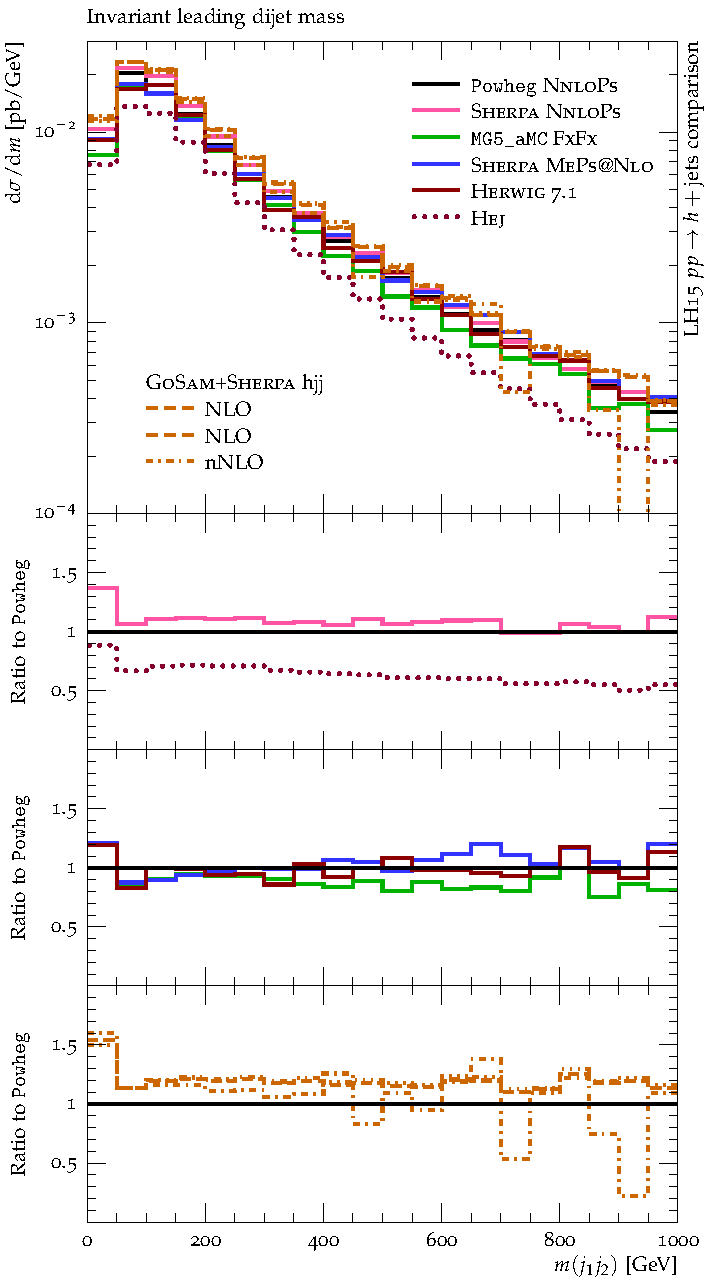
\includegraphics[width=0.47\textwidth]{figures/hjetscomp_u_dijet_mass.pdf}
  \hfill
  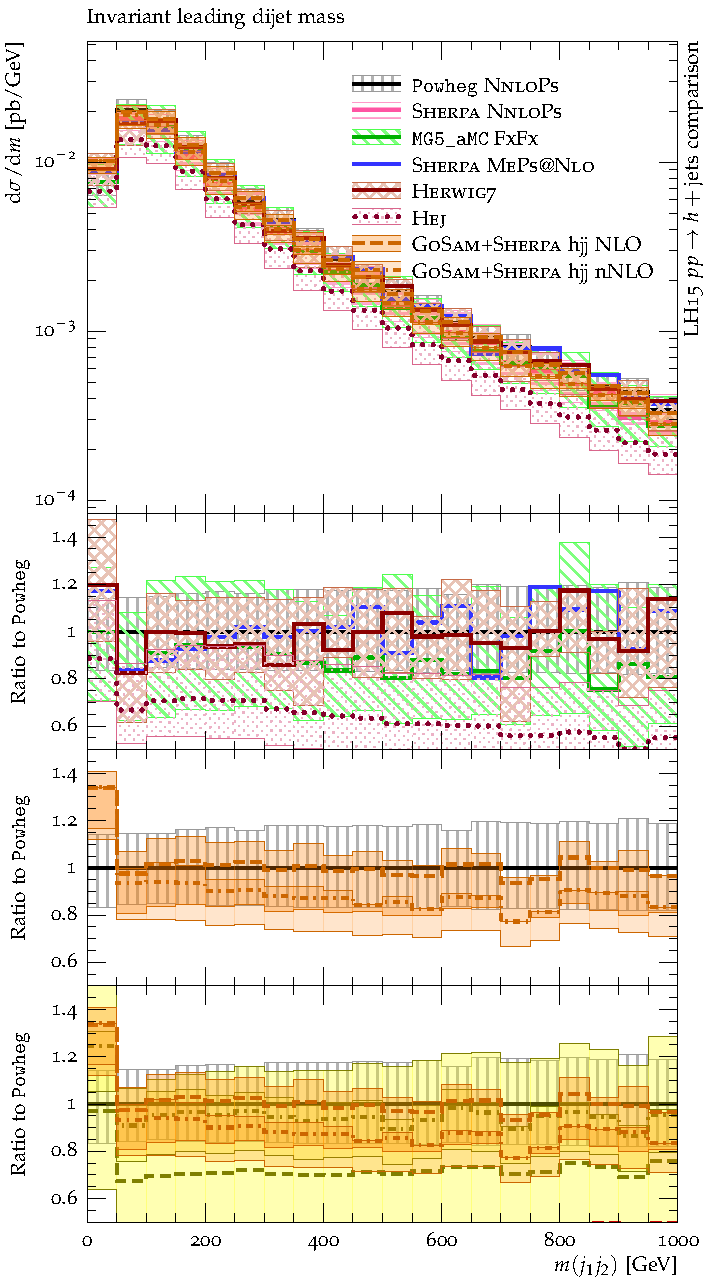
\includegraphics[width=0.47\textwidth]{figures/hjetscomp_dijet_mass.pdf}
  \caption{
    The invariant mass of the leading dijet system without (left) and
    with (right) uncertainties.
    \label{fig:higgscomp:results:2obs:mjj}
  }
\end{figure}

The rapidity separation between the leading and sub-leading jets is
shown in Figure~\ref{fig:higgscomp:results:2obs:dyjj}, for $H+\ge2$
jets. MG5 is lower than Powheg at high $\Delta y$ (while Sherpa is
slightly higher).  Powheg is in good agreement with the fixed order
gosam results for $H+\ge2$ jets. Similar conclusions hold for for the
dijet mass distribution, as shown in
Figure~\ref{fig:higgscomp:results:2obs:mjj}, although the differences
among predictions are smaller.

\begin{figure}[t!]
  \centering
  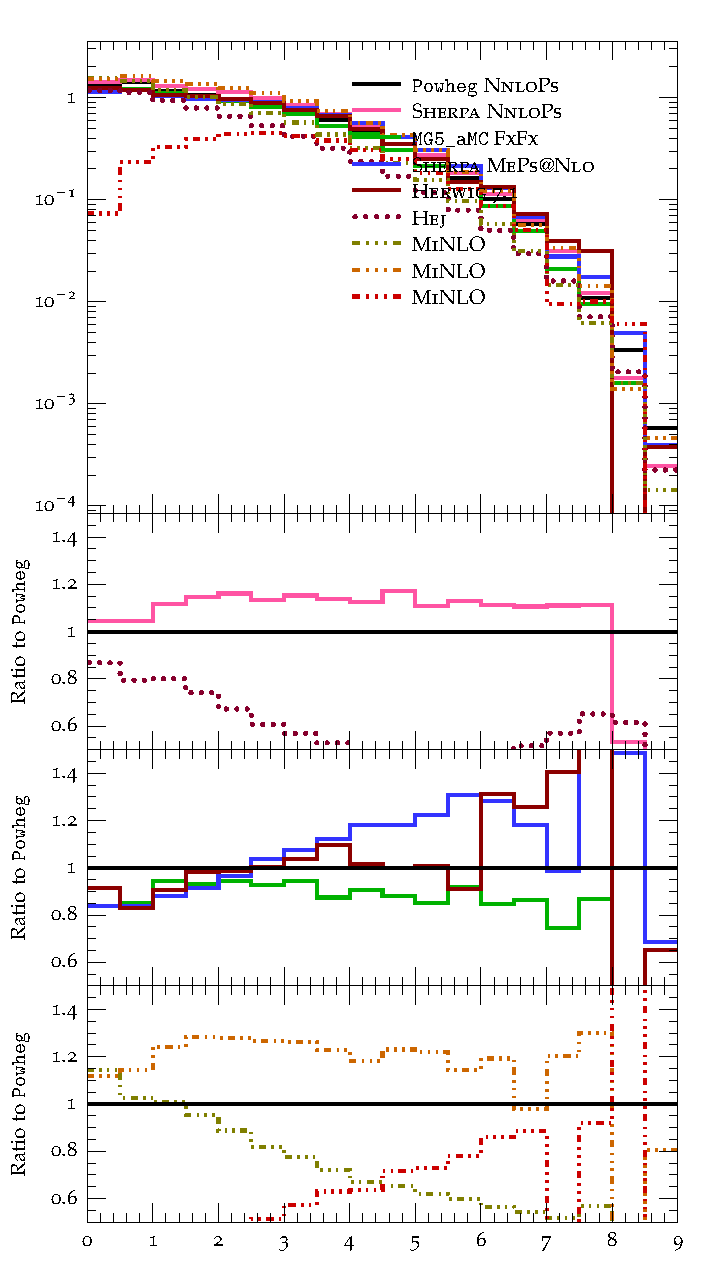
\includegraphics[width=0.47\textwidth]{figures/hjetscomp_u_jjfb_dy.pdf}
  \hfill
  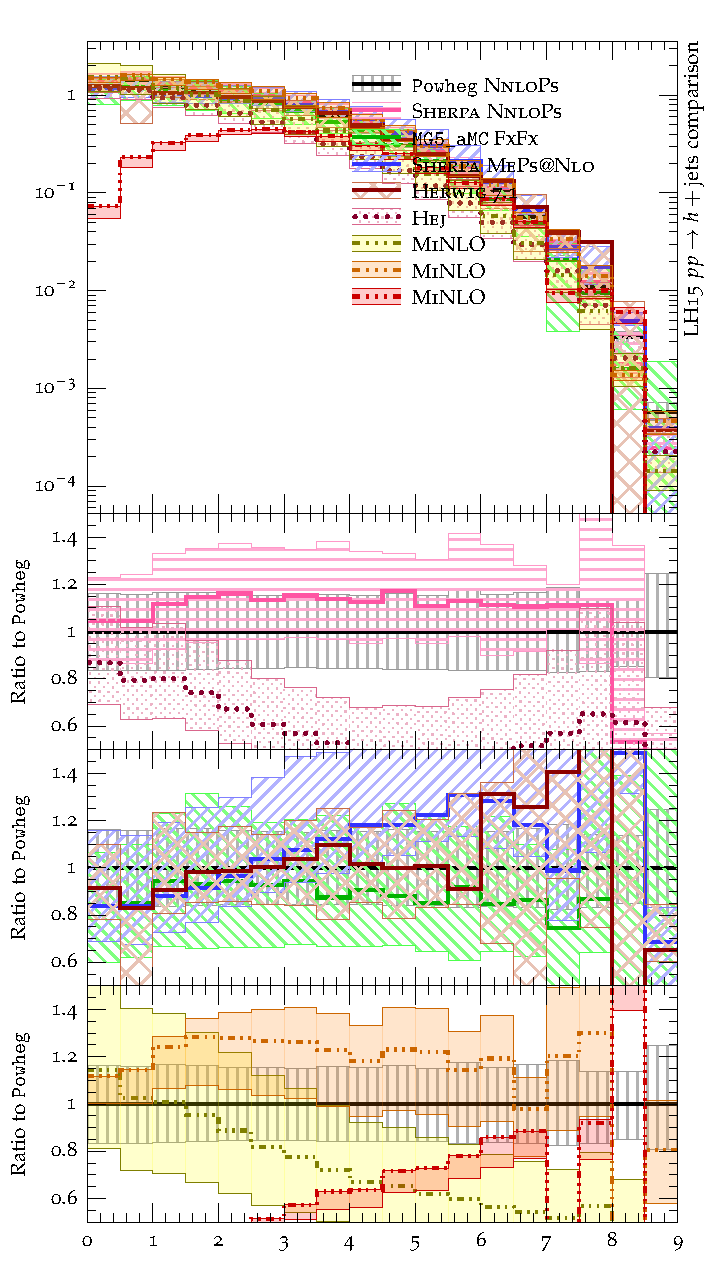
\includegraphics[width=0.47\textwidth]{figures/hjetscomp_jjfb_dy.pdf}
  \caption{
    The rapidity separation between the two most forward-backward jets
    for $H+\ge2$ jets, without (left) and with (right) uncertainties. 
    \label{fig:higgscomp:results:2obs:dyjj_fb}
  }
\end{figure}

The rapidity separation between the two most forward-backward jets is
shown in Figure~\ref{fig:higgscomp:results:2obs:dyjj_fb}. As for the
$p_T$-ordered distribution, MG5 is lower than Powheg at high $\Delta
y$ while Sherpa is higher. Powheg now has a slope compared to the
Gosam NLO results, but, interestingly, not compared to the nNLO
results.

\begin{figure}[t!]
  \centering
  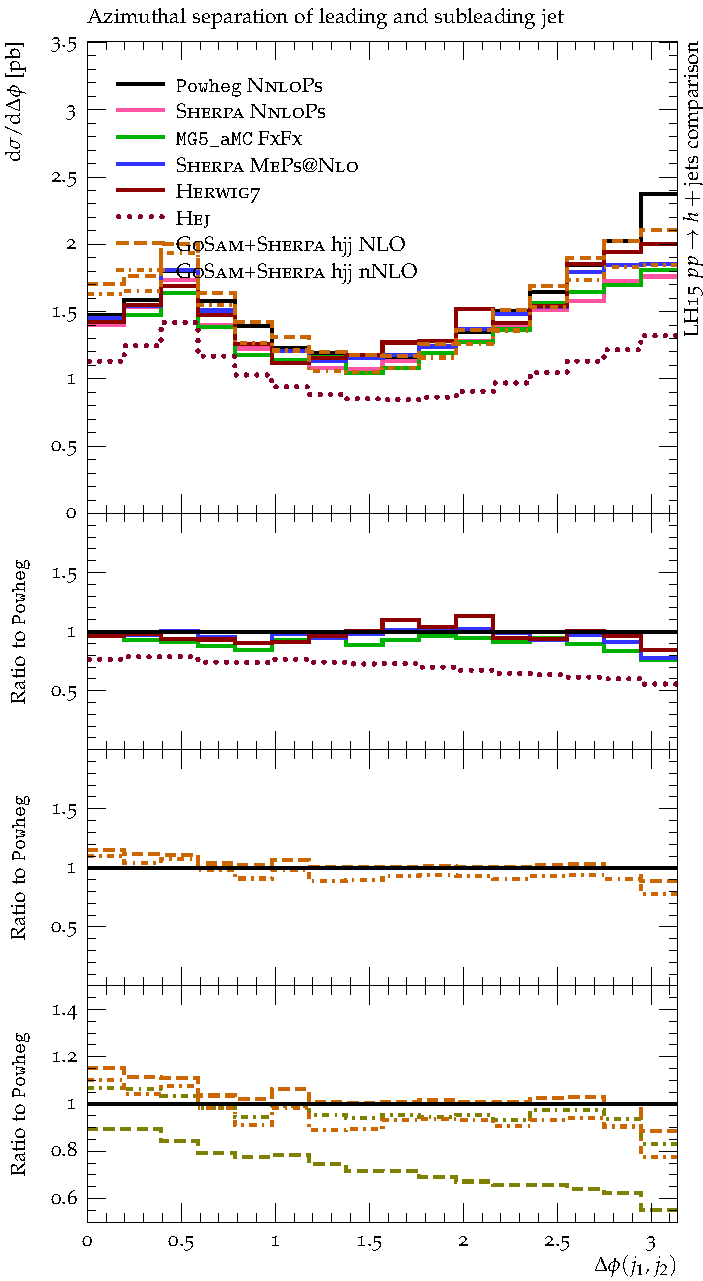
\includegraphics[width=0.47\textwidth]{figures/hjetscomp_u_deltaphi_jj_incl.pdf}
  \hfill
  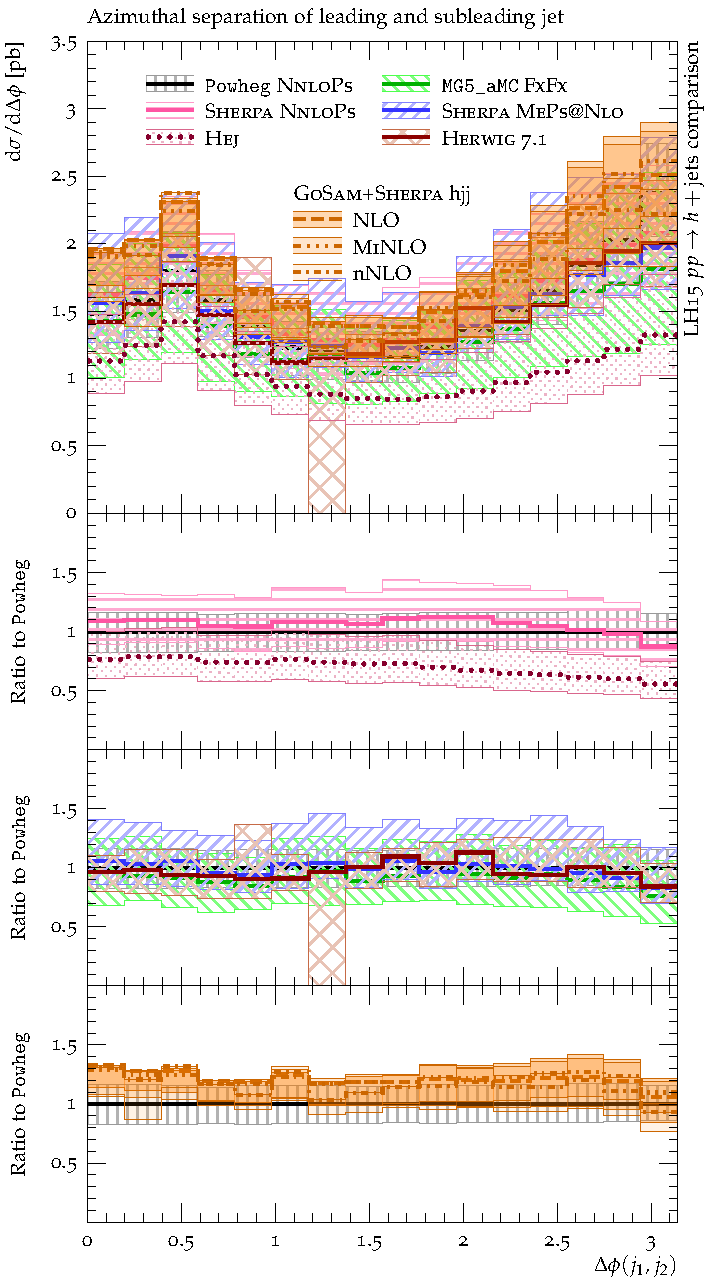
\includegraphics[width=0.47\textwidth]{figures/hjetscomp_deltaphi_jj_incl.pdf}
  \caption{
    The $\Delta\phi$ separation between the two leading jets for
    $H+\ge2$ jets, without (left) and with (right) uncertainties. 
    \label{fig:higgscomp:results:2obs:dphi_jj}
  }
\end{figure}

The $\Delta\phi$ separation between the two leading jets is shown in
Figure~\ref{fig:higgscomp:results:2obs:dphi_jj}. All predictions are
in good agreement with each other, except for HEJ, which has a leading
order normalization. Similar distributions (and agreement) are
observed if the two most forward-backward jets are chosen instead.



\clearpage
\subsection{VBF observables}
\label{sec:hjetscomp:results:VBFobs}

To single out observables with VBF kinematics, additional cuts are
placed, requiring the dijet mass distribution formed from the leading
and sub-leading jets to have a mass greater than 400 GeV, and in
addition requiring the two leading jets to have a rapidity separation
greater than 2.8 (VBF cuts). An alternative set of cuts requires that
any two jets satisfy the preceding criteria (VBF2 cuts).

\begin{figure}[t!]
  \centering
  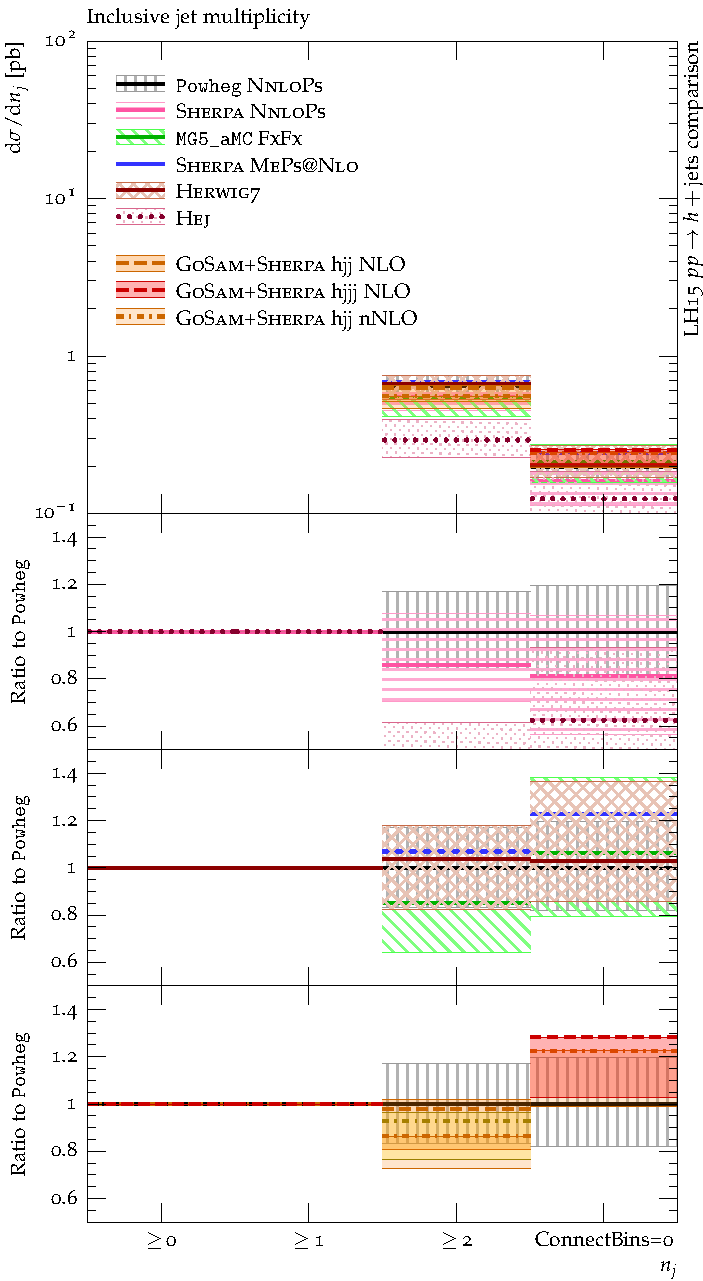
\includegraphics[width=0.47\textwidth]{figures/hjetscomp_NJet_incl_30_VBF.pdf}
  \hfill
  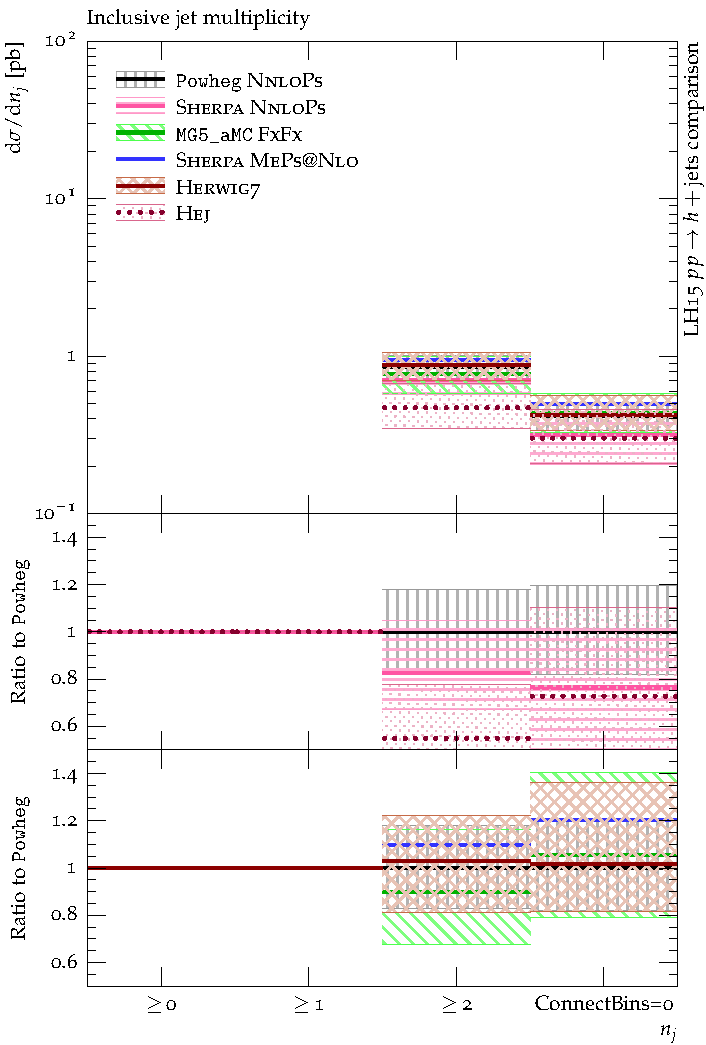
\includegraphics[width=0.47\textwidth]{figures/hjetscomp_NJet_incl_30_VBF2.pdf}
  \caption{\label{fig:higgscomp:results:inclobs:njets_VBF}
    The inclusive jet multiplicities with VBF (left) and VBF2 (right)
    cuts.  }
\end{figure}

The inclusive jet multiplicity distributions with VBF cuts are shown
in Figure~\ref{fig:higgscomp:results:inclobs:njets_VBF}. The hierarchy
is essentially the same as for the inclusive jet multiplicity
distribution without any cuts. The differences among the predictions
are somewhat smaller with the VBF2 cuts than with the VBF cuts.

\begin{figure}[t!]
  \centering
  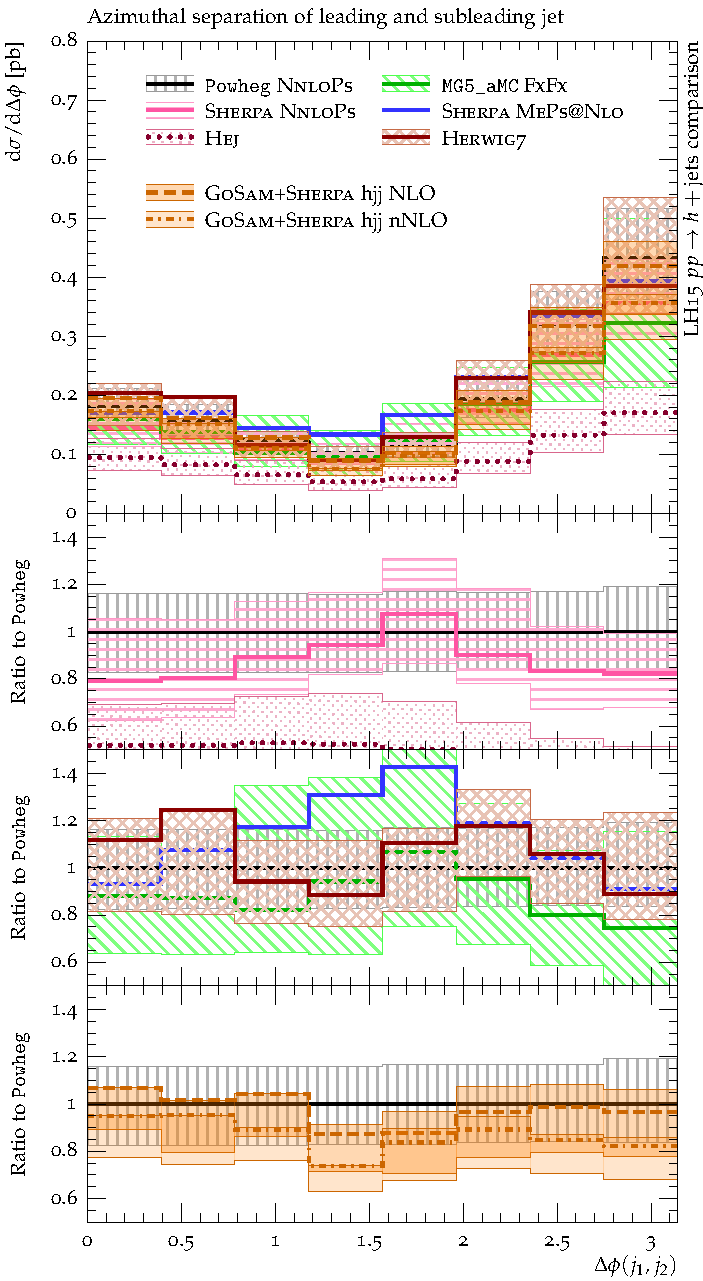
\includegraphics[width=0.47\textwidth]{figures/hjetscomp_deltaphi_jj_VBF.pdf}
  \hfill
  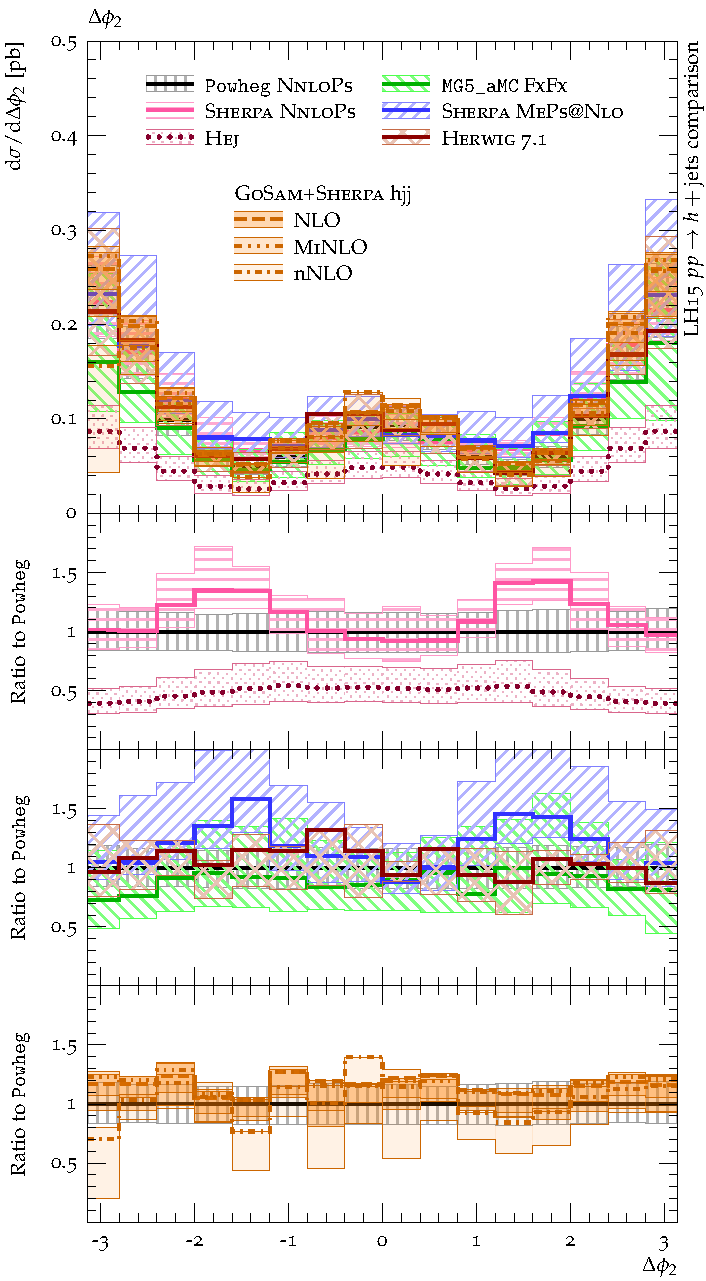
\includegraphics[width=0.47\textwidth]{figures/hjetscomp_deltaphi2_VBF.pdf}
  \caption{
    Azimuthal separation of the leading jet pair (left) and 
    $\Delta\phi_2$ (right) after applying VBF cuts in $H+\ge2$ jet
    production.
    \label{fig:higgscomp:results:VBFobs:dphijj_phi2}
    \Todo{Joey suggests to add no-uncertainty plot versions here too.}
  }
\end{figure}

The $\Delta\phi$ separation between the two leading jets applying the
VBF cuts is shown in
Figure~\ref{fig:higgscomp:results:VBFobs:dphijj_phi2}. All predictions
are in reasonable agreement with each other, although not as good
agreement as for the inclusive case. Similar distributions (and
agreement) are observed if the two most forward-backward jets are
chosen instead.

\Todo{I'm not sure what other observables to put into this section. It
  would have been nice to have the 3rd jet pT distribution with VBF
  cuts.}



\clearpage
\subsection{Multijet observables}
\label{sec:hjetscomp:results:mjobs}

\begin{figure}[t!]
  \centering
  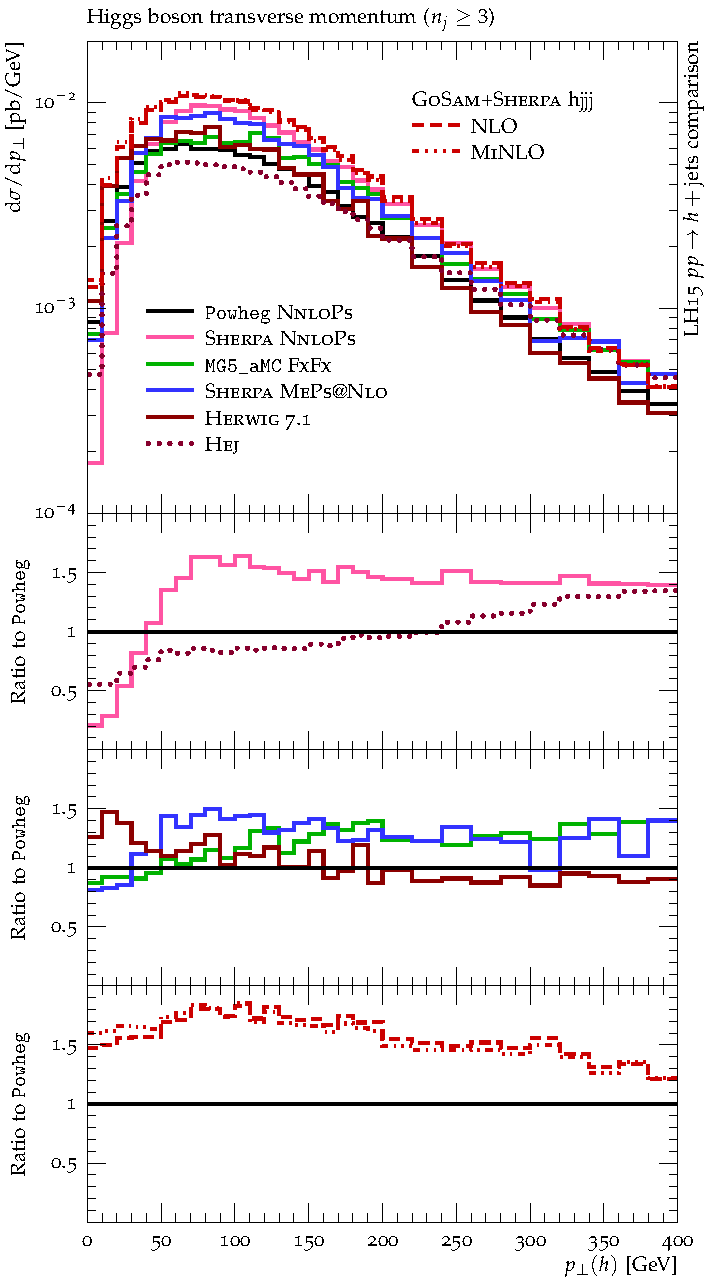
\includegraphics[width=0.47\textwidth]{figures/hjetscomp_u_H_jjj_pT_incl.pdf}
  \hfill
  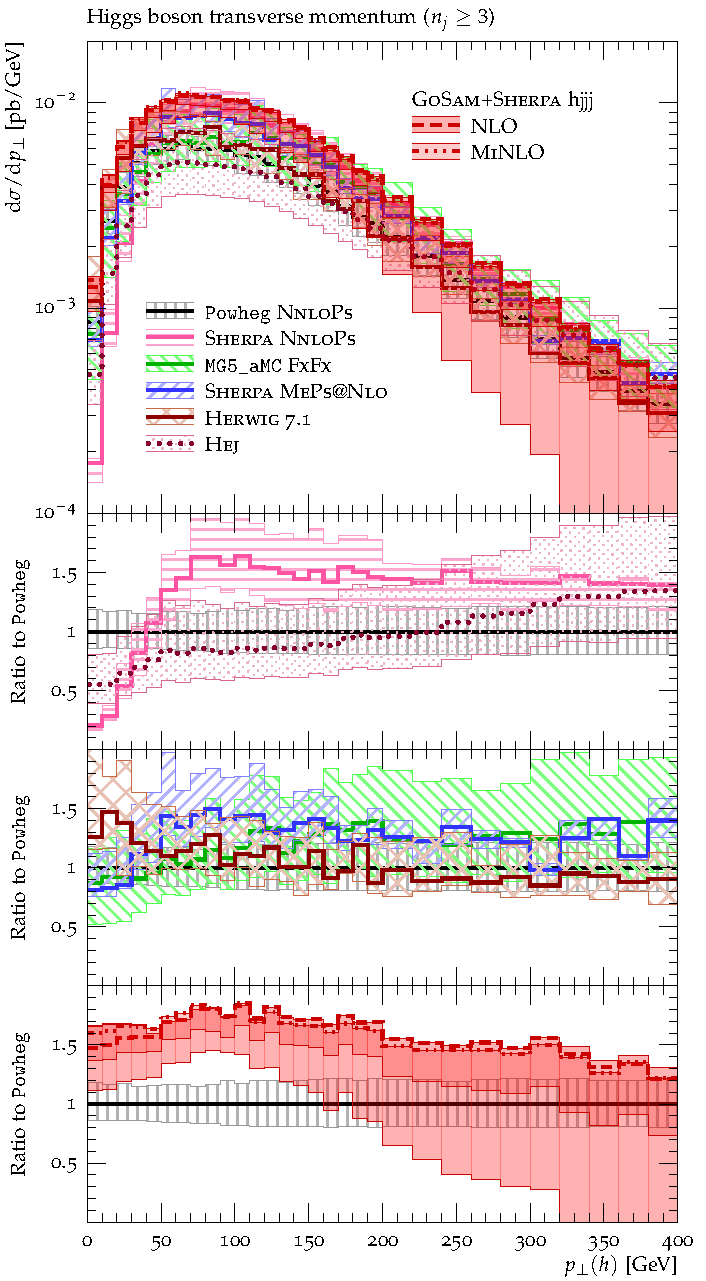
\includegraphics[width=0.47\textwidth]{figures/hjetscomp_H_jjj_pT_incl.pdf}
  \caption{
    The Higgs boson transverse momentum in the presence of at least three 
    jets, shown without (left) and with (right) theoretical uncertainties.
    \label{fig:higgscomp:results:mobs:hpt_j3}
  }
\end{figure}

The Higgs boson transverse momentum distribution for $H+\ge3$ jets is
shown in Figure~\ref{fig:higgscomp:results:mobs:hpt_j3}. MG5 and
Sherpa tend to be higher than Powheg (where the jet is produced by a
parton shower), and similar to that from Gosam $H+\ge3$ jets, which
has the correct NLO $K$-factor.

\begin{figure}[t!]
  \centering
  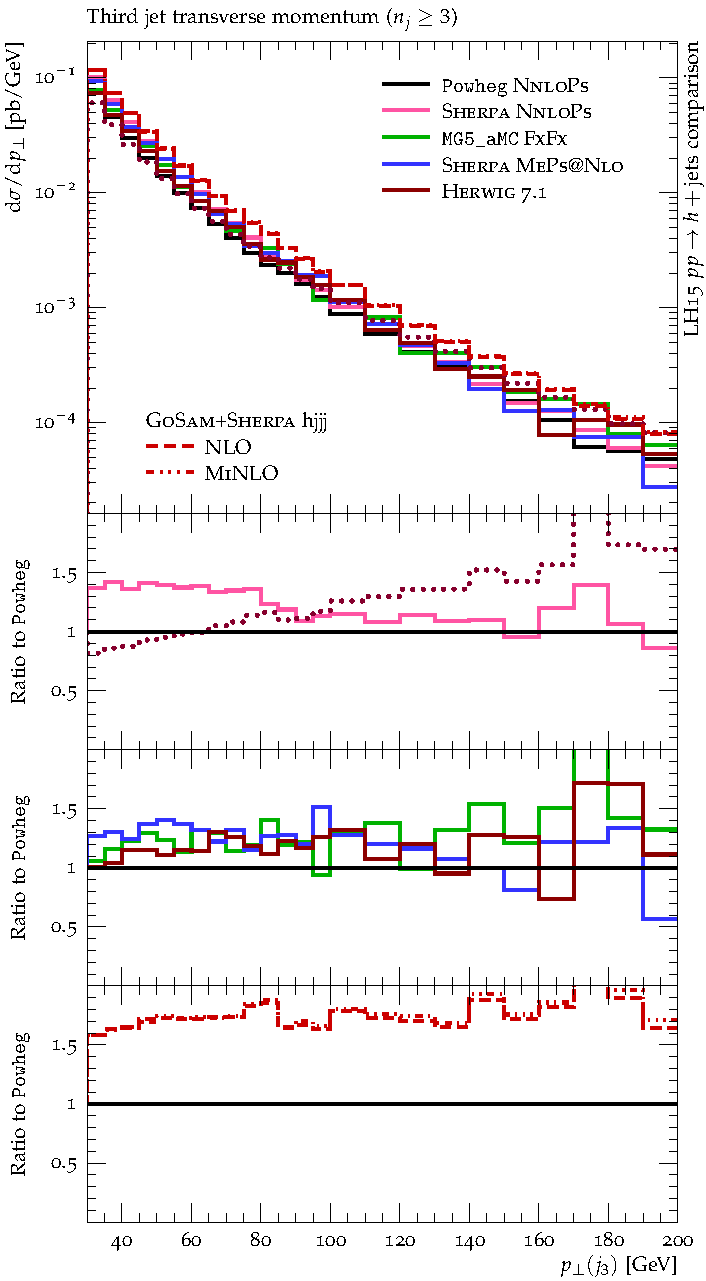
\includegraphics[width=0.47\textwidth]{figures/hjetscomp_u_jet3_pT_incl.pdf}
  \hfill
  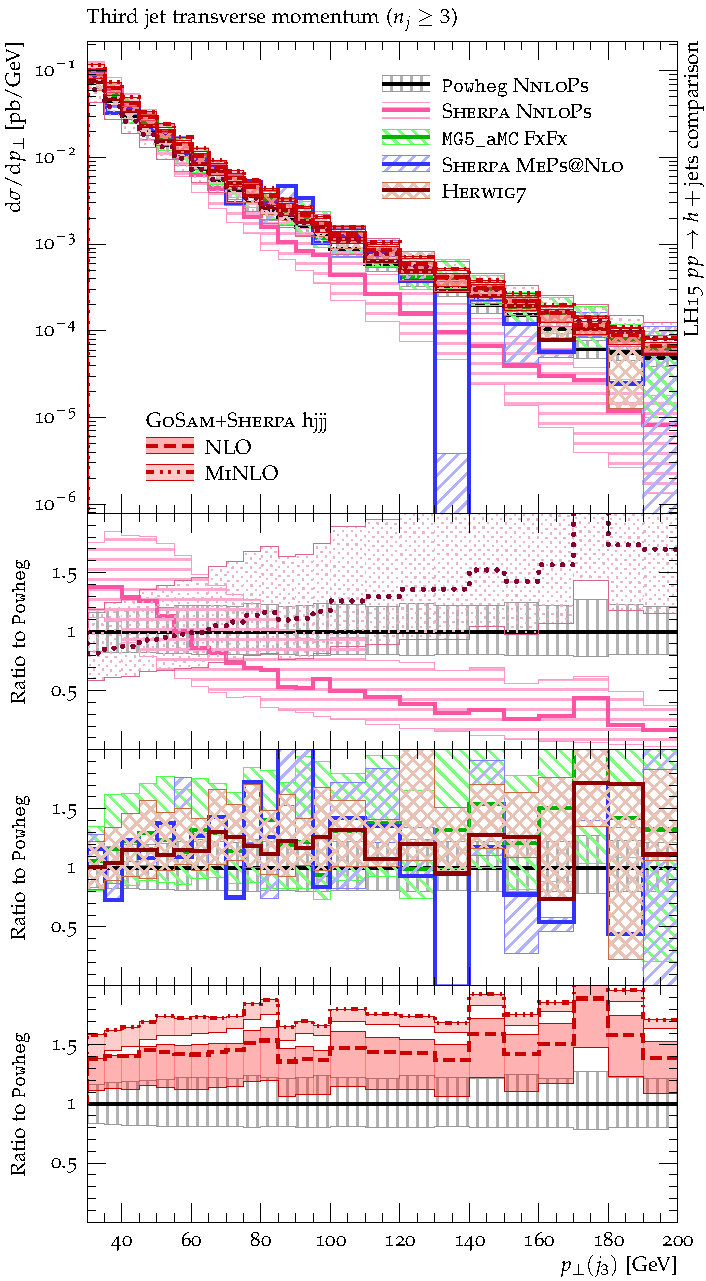
\includegraphics[width=0.47\textwidth]{figures/hjetscomp_jet3_pT_incl.pdf}
  \caption{
    The third jet transverse momentum distribution for $H+\ge3$ jets
    shown without (left) and with (right) theoretical uncertainty bands.
    \label{fig:higgscomp:results:mobs:j3pt}
  }
\end{figure}

The third jet $p_T$ for $H+\ge3$ jets is shown in
Figure~\ref{fig:higgscomp:results:mobs:j3pt}. MG5, Herwig7 and Sherpa
tend to be higher than Powheg (where the jet is produced by a parton
shower), but lower than that from Gosam $H+\ge3$ jets, which has the
correct NLO $K$-factor. The multijet phase space results in smaller
Sudakov effects, and thus better agreement with the fixed-order
predictions.

\begin{figure}[t!]
  \centering
  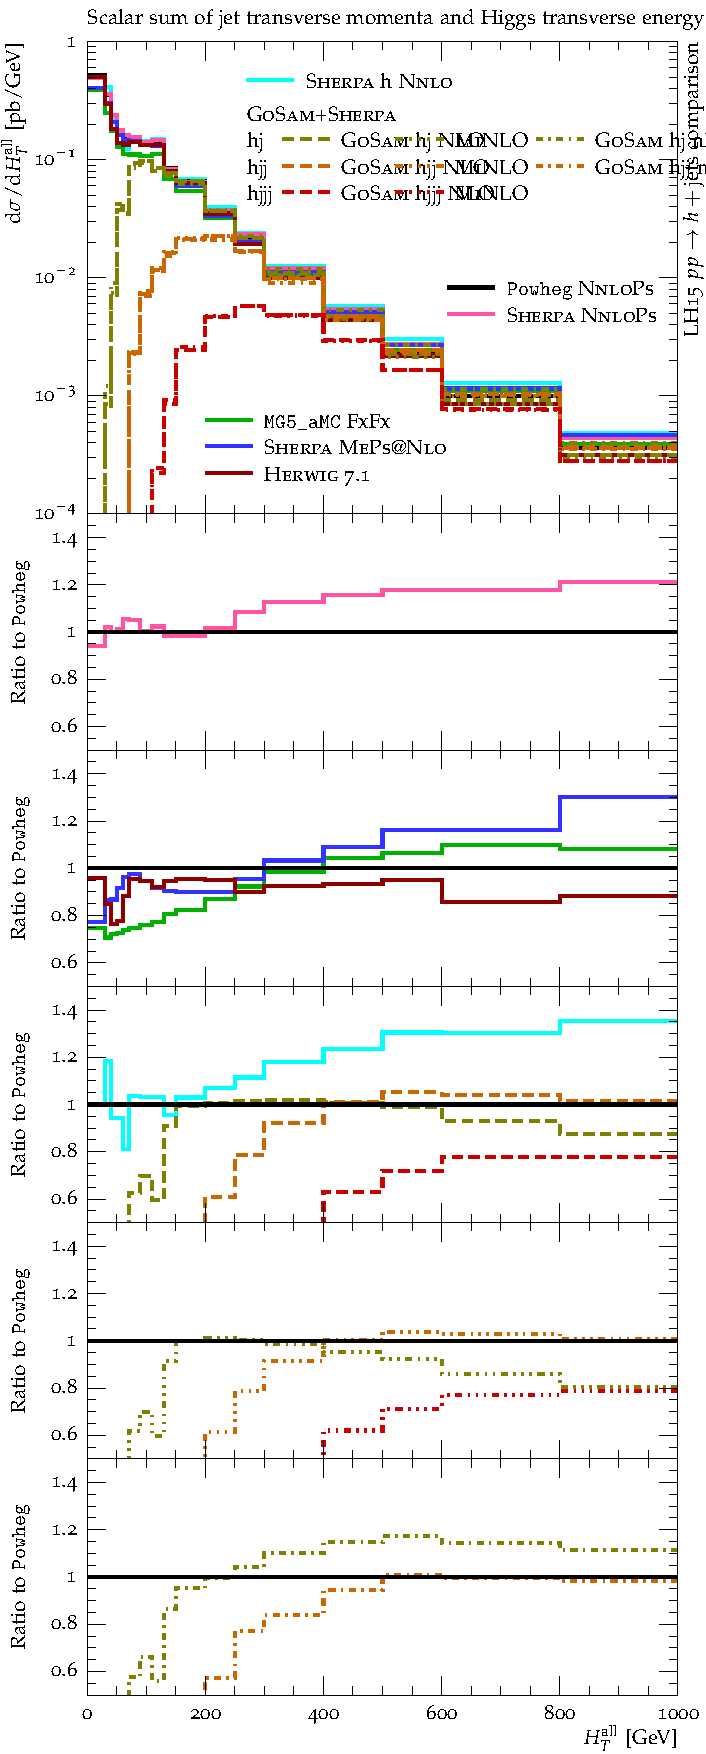
\includegraphics[width=0.47\textwidth]{figures/hjetscomp_u_HT_all.pdf}
  \hfill
  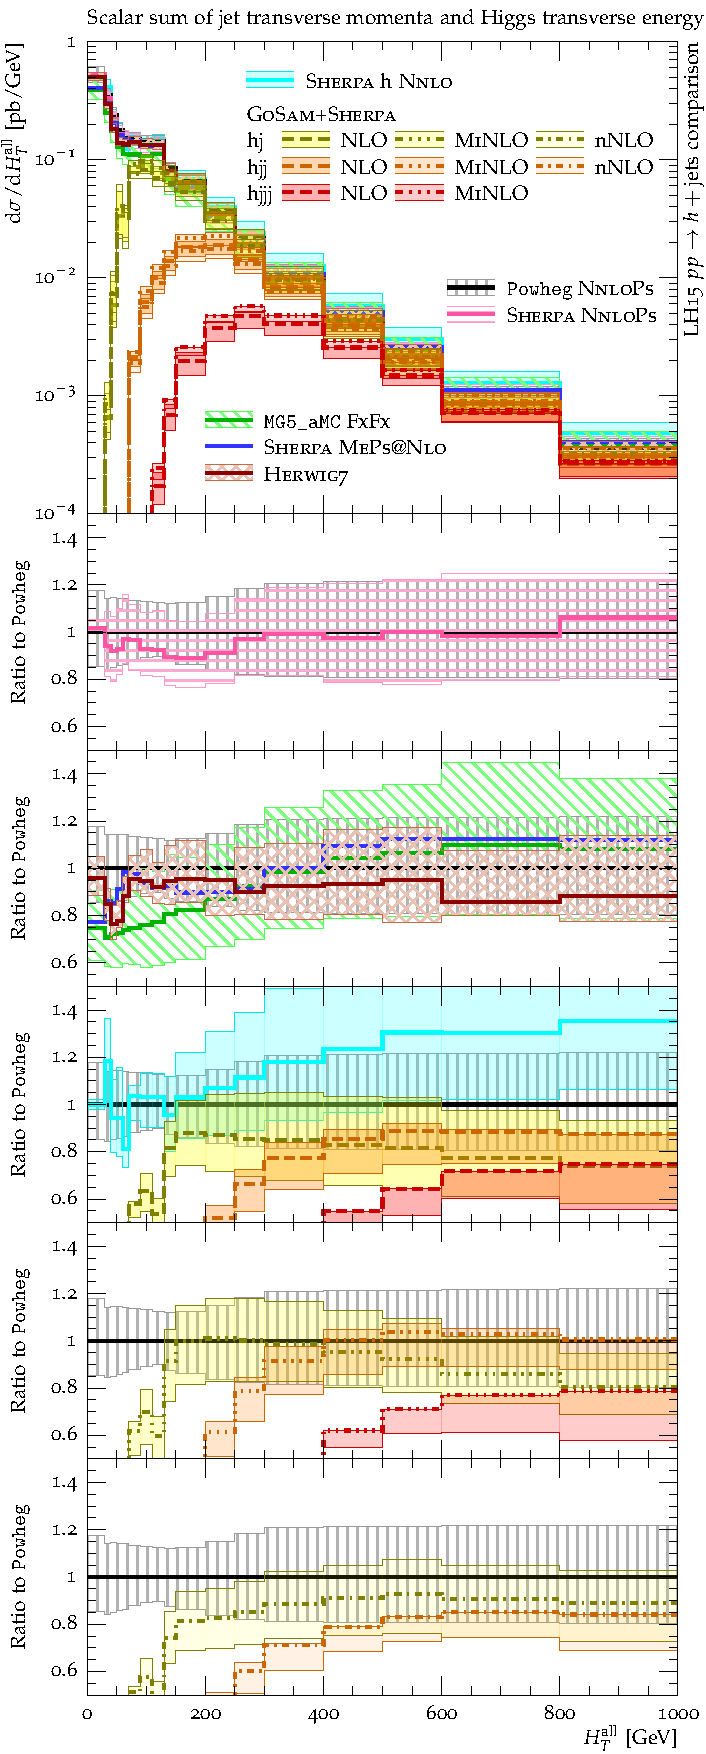
\includegraphics[width=0.47\textwidth]{figures/hjetscomp_HT_all.pdf}
  \caption{
    The $H_T$ distribution for $H+\ge1$ jets \Todo{is this correct?}
    without (left) and with (right) uncertainties.
    \label{fig:higgscomp:results:mobs:HT_all}
  }
\end{figure}

\begin{figure}[t!]
  \centering
  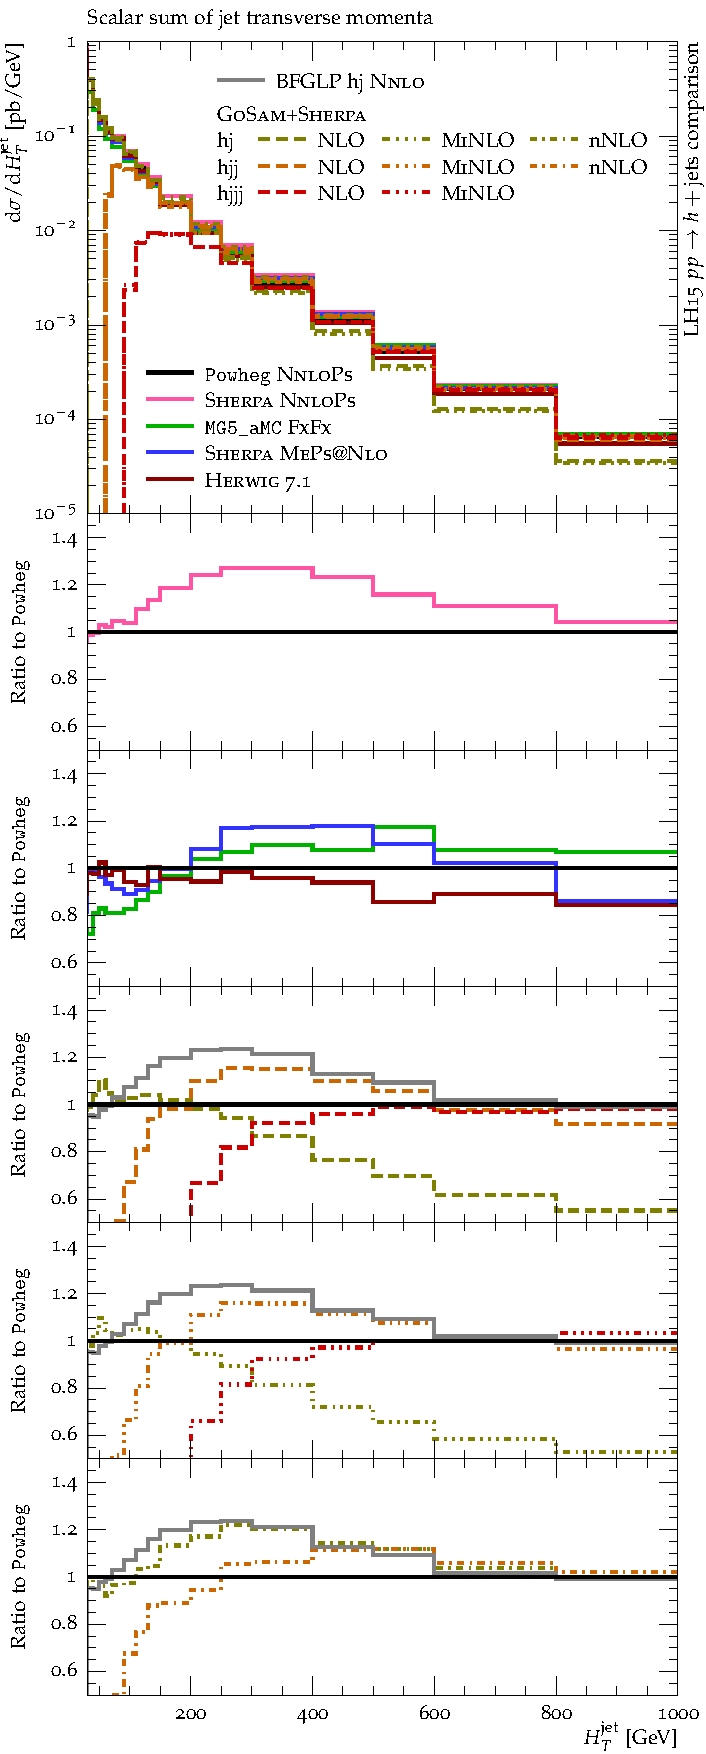
\includegraphics[width=0.47\textwidth]{figures/hjetscomp_u_HT_jets.pdf}
  \hfill
  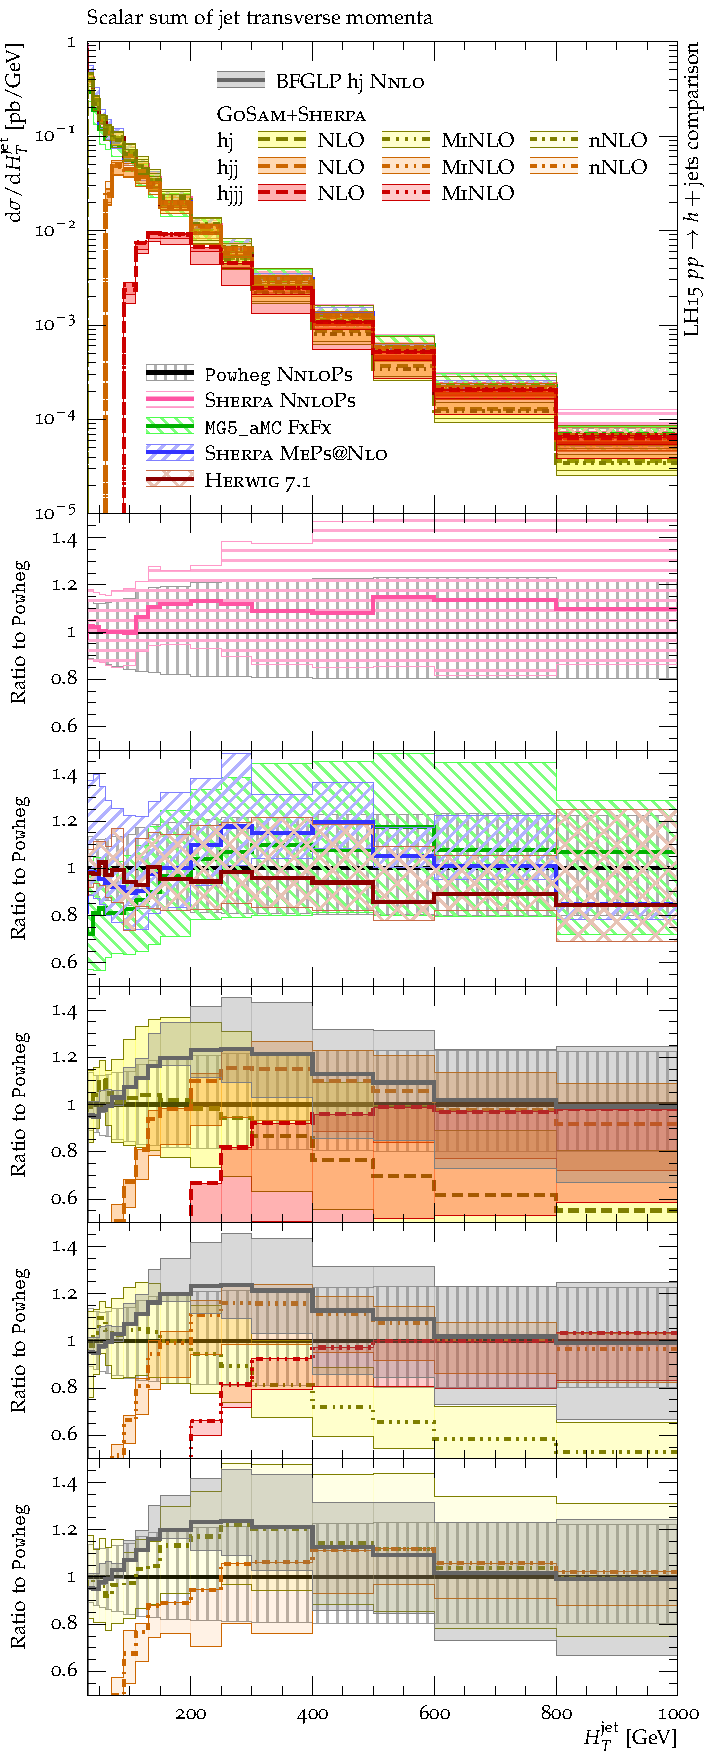
\includegraphics[width=0.47\textwidth]{figures/hjetscomp_HT_jets.pdf}
  \caption{
    The $H_{T,\mathrm{jets}}$ distribution for $H+\ge1$ jet final
    states, without (left) and with (right) uncertainties.
    \label{fig:higgscomp:results:mobs:HT_jets}
  }
\end{figure}

The $H_T$ distribution (sum of the transverse momenta for all objects
in the final state) for $H+\ge1$ jets is shown in
Figure~\ref{fig:higgscomp:results:mobs:HT_all} and the $H_T$
distribution for jets only is shown in in
Figure~\ref{fig:higgscomp:results:mobs:HT_jets}. \Todo{Jan: we don't
  consider $H$ decays, so the all-objects HT would be different from
  an experimental point of view. Do we want both HTs and clarify or
  only the HTjets.}
MG5 and Sherpa tend to be lower than Powheg at low $H_T$ and higher at
large $H_T$. The fixed order predictions (from gosam and from $H+\ge1$
jet at NNLO) are consistently lower than Powheg (although the NNLO
prediction does agree with Powheg in the 150-300 GeV range for
$HT_{jets}$).



\clearpage
\subsection{Jet veto cross sections}
\label{sec:hjetscomp:results:jvobs}

This section is concerned with the cummulative jet veto cross sections. 
In the first three cases, Figures 
\ref{fig:higgscomp:results:jvobs:jvxs0}-\ref{fig:higgscomp:results:jvobs:jvxs1j200}, 
additional radiation is vetoed by means of a maximal transverse 
momentum of the (sub)leading jet, $p_\perp^\text{veto}$. These 
observables recover the respective inclusive cross section as 
$p_\perp^\text{veto}\to\infty$. In this region, the fixed order 
part of the respective calculations dominates the cross section 
and associated uncertainties. The opposite regime, $p_\perp^\text{veto}\to 0$, 
is a classic example of a resummation dominated observable. Here, the 
properties of the respective parton showers come fully into play and 
differences are largely due to their characteristics. The last case 
investigated is cross section after VBF cuts when vetoing additional 
central jet activity in dependence of the rapidity distance of the 
tagging jet pair, $y_\text{dist}<y_\text{dist}^\text{max}$. Here, 
DGLAP-type resummation regions are present throughout the spectrum and 
this observable should be ideal to study BFKL-like dynamics.

\begin{figure}[t!]
  \centering
  \includegraphics[width=0.47\textwidth]{figures/hjetscomp_u_xs_jet_veto_j0.pdf}
  \hfill
  \includegraphics[width=0.47\textwidth]{figures/hjetscomp_xs_jet_veto_j0.pdf}
  \caption{
    The exclusive zero jet cross section as a function of 
    the vetoed minimal leading jet transverse momentum,
    without (left) and with (right) uncertainties.
    \label{fig:higgscomp:results:jvobs:jvxs0}
  }
\end{figure}

We start by considering 
the cross section for the production of a Higgs boson and no 
additional jets as a function of the minimum jet transverse momentum 
is shown in Figure~\ref{fig:higgscomp:results:jvobs:jvxs0}. Remarkable 
agreement between both \NNLOPS simulations and the dedicated resummation 
of STWZ is found, typically well with 5\% within the considered range. 
However, as both \NNLOPS' resummation accuracy is limited by their parton 
shower's accuracy and both do not (\Powheg) or only partially (\Sherpa) 
assess their intrinsic uncertainty and interplay with the hard process' 
scale variations, their uncertainties remain much larger than those of 
STWZ. The multijet merged calculations show a wider spread. In addition to 
suffering from their NLO normalisation in the $p_\perp^\text{veto}\to\infty$ 
limit, they show different behaviour as $p_\perp^\text{veto}\to 0$. Here, 
\Sherpa \MEPSatNLO exhibits more QCD activity than the other computations. 

\begin{figure}[t!]
  \centering
  \includegraphics[width=0.47\textwidth]{figures/hjetscomp_u_xs_jet_veto_j1_30.pdf}
  \hfill
  \includegraphics[width=0.47\textwidth]{figures/hjetscomp_xs_jet_veto_j1_30.pdf}
  \caption{
    The cross section for events containing a Higgs boson 
    and one jet with $p_\perp>30\,\gev$ as a function of
    the vetoed minimal second jet transverse momentum without
    (left) and with (right) uncertainties.
    \label{fig:higgscomp:results:jvobs:jvxs1j30}
  }
\end{figure}

\begin{figure}[t!]
  \centering
  \includegraphics[width=0.47\textwidth]{figures/hjetscomp_u_xs_jet_veto_j1_200.pdf}
  \hfill
  \includegraphics[width=0.47\textwidth]{figures/hjetscomp_xs_jet_veto_j1_200.pdf}
  \caption{
    The cross section for events containing a Higgs boson 
    and one jet with $p_\perp>200\,\gev$ as a function of
    the vetoed minimal second jet transverse momentum without
    (left) and with (right) uncertainties.
    \label{fig:higgscomp:results:jvobs:jvxs1j200}
  }
\end{figure}

Next, we require the presence of at least one jet with 
a minimal transverse momentum of $30$ and $200$ \gev, respectively. 
The cross section as a function of 
the sub-leading jets maximal transverse momentum is displayed in 
Figure~\ref{fig:higgscomp:results:jvobs:jvxs1j30} and 
Figure~\ref{fig:higgscomp:results:jvobs:jvxs1j200}, respectively. 
Before starting the discussion it worthy to note that although all parton 
shower matched or merged calculations have the same accuracy as 
$p_\perp^\text{veto}\to\infty$ and in the resummation dominated region, 
the multijet merged calculation possess a better description of the 
second jet emission and thus should lead to more accurate results 
throughout the spectrum provided the merging systematics are under control. 
Currently employed uncertainty estimates, however, will not reflect this 
as resummation uncertainties are not assessed or only incompletely assessed.

Putting no special requirements on the leading jet, cf.\ Figure 
\ref{fig:higgscomp:results:jvobs:jvxs1j30}, good agreement 
between all calculations is found. The \NNLOPS ones agreen again within 
5\% of one another with very similar uncertainties. This is noteworthy 
in sofar as, in comparison with the results of 
Figure~\ref{fig:higgscomp:results:jvobs:jvxs0}, both calculations' 
accuracies have degraded by one order. The multijet merged calculations 
also show a similar behaviour as in the previous case, also showing the 
same features as before: \MGaMC exhibits a smaller cross section due to 
its scale choice while \Sherpa \MEPSatNLO predicts more soft radiation. 
Only the slight relative lack of small $p_\perp$ radiation is more 
pronounced in \Herwig now. Again, the uncertainties of \MGaMC and \Sherpa 
are of similar size while \Herwig's are somewhat smaller than the \NNLOPS 
ones, especially in the resummation dominated region as 
$p_\perp^\text{veto}\to 0$.

Raising the requirements on the leading jet to $200$ \gev in Figure 
\ref{fig:higgscomp:results:jvobs:jvxs1j200} now shows clear distinctions 
between the different calculations now. Among the \NNLOPS calculations, 
\Sherpa starts out at a higher asymtotic cross section but remains within 
20\% and of \Powheg, the respective uncertainties covering one another. 
The multijet merged calculations show \Herwig largely agreeing with 
\Powheg with a constant offset of $-10\%$ and the familiar lower 
probability of low-$p_\perp$ jet emissions. \Sherpa \MEPSatNLO's 
asymtotic cross section is as large as the \Sherpa \NNLOPS one and, 
unsurprisingly due to the use of the same parton shower, shows a 
similar radiation pattern for a large range. As before, it exhibits 
a relative overabundance of soft jet radiation. Lastly, \MGaMC's 
asymtotic cross section now is the same level as \Powheg's, despite 
its higher scale choice. The pattern of the uncertainties, however, 
remains the same as before.

\begin{figure}[t!]
  \centering
  \includegraphics[width=0.47\textwidth]{figures/hjetscomp_u_xs_central_jet_veto_VBF.pdf}
  \hfill
  \includegraphics[width=0.47\textwidth]{figures/hjetscomp_xs_central_jet_veto_VBF.pdf}
  \caption{
    The cross section after VBF cuts as a function of the rapidity
    distance of the two ($p_T$-ordered) tagging jets. A veto has been
    applied on the leading central jet with transverse momentum larger
    than 30~GeV.
    \label{fig:higgscomp:results:jvobs:cjvxsvbf}
  }
\end{figure}

Finally, we consider the cross section after VBF cuts applying a veto 
on additional central jet activity with $p_\perp>30\,\gev$ in dependence 
of the maximal rapidity distance of the tagging jets, 
$y_\text{dist}<y_\text{dist}^\text{max}$. Here, all parton shower based 
resummation calculations give very similar results with \MGaMC possessing 
a reduced cross section due to its scale choice. \Hej, being based on 
BFKL dynamics, does not deviate substantially in its predicted shape. 
However, its cross section is reduced by a constant 50-60\%.
